%% FEUP THESIS STYLE for LaTeX2e
%% how to use feupteses for MIEIC dissertations
%%
%% FEUP, JCL & JCF,  Wed Oct  4 16:32:24 2017
%%
%% PLEASE send improvements to jlopes at fe.up.pt and to jcf at fe.up.pt
%%

%%========================================
%% Commands: pdflatex thesis
%%           bibtex thesis
%%           makeindex thesis (only if creating an index) 
%%           pdflatex thesis
%% Alternative:
%%          latexmk -pdf thesis.tex
%%========================================

\documentclass[11pt,a4paper,twoside,openright]{report}
\usepackage[utf8]{inputenc}
%\usepackage[latin1]{inputenc}

%%%%%%% English version 

%% MIEIC options
% \usepackage[mieic]{feupteses}                  % work version
\usepackage[mieic,juri]{feupteses}             % juri verrion
%\usepackage[mieic,final]{feupteses}            % final version

%% Additional options for feupteses.sty: 
%% - portugues: titles, etc in portuguese
%% - onpaper: links are not shown (for paper versions)
%% - backrefs: include back references from bibliography to citation place

%%%%%%% Portuguese version

%\usepackage[mieic,portugues]{feupteses}        % work version
%\usepackage[mieic,portugues,juri]{feupteses}   % juri version
%\usepackage[mieic,portugues,final]{feupteses}  % final version

%% Uncomment the next lines if side by side graphics used
% \usepackage[lofdepth,lotdepth]{subfig}
\usepackage{graphicx}
\usepackage{float}
\usepackage{subcaption}

%Bar chart drawing library 
\usepackage{pgfplots} 

%tables span multiple pages
\usepackage{longtable}

%Multiple footnotes at same point
\usepackage[multiple]{footmisc}

%% Include color package
\usepackage{hyperref,xcolor}
\definecolor{cloudwhite}{cmyk}{0,0,0,0.025}
\definecolor{engineering}{rgb}{0.549, 0.176, 0.098}
\hypersetup {
    colorlinks=true,
    linkcolor=engineering,
    urlcolor={engineering},
    filecolor={engineering},
    citecolor={engineering},
    allcolors={engineering}
}

%% Include source-code listings package
\usepackage{listings}
\lstset{ %
 language=C,                        % choose the language of the code
 basicstyle=\footnotesize\ttfamily,
 keywordstyle=\bfseries,
 numbers=left,                      % where to put the line-numbers
 numberstyle=\scriptsize\texttt,    % the size of the fonts that are used for the line-numbers
 stepnumber=1,                      % the step between two line-numbers. If it's 1 each line will be numbered
 numbersep=8pt,                     % how far the line-numbers are from the code
 frame=tb,
 float=htb,
 aboveskip=8mm,
 belowskip=4mm,
 backgroundcolor=\color{cloudwhite},
 showspaces=false,                  % show spaces adding particular underscores
 showstringspaces=false,            % underline spaces within strings
 showtabs=false,                    % show tabs within strings adding particular underscores
 tabsize=2,	                    % sets default tabsize to 2 spaces
 captionpos=b,                      % sets the caption-position to bottom
 breaklines=true,                   % sets automatic line breaking
 breakatwhitespace=false,           % sets if automatic breaks should only happen at whitespace
 escapeinside={\%*}{*)},            % if you want to add a comment within your code
 morekeywords={*,var,template,new}  % if you want to add more keywords to the set
}

%% Allow for better aligning of equations
\usepackage{amsmath}

\usepackage{dirtytalk}

\usepackage{enumitem}

\usepackage{lscape}
\usepackage{graphicx}

\usepackage{tabularx}

%% Rotate images (for big horizontal)
\usepackage{rotating}

\usepackage{placeins} % Prevent images from being placed outside of their section

\let\Oldsection\section
\renewcommand{\section}{\FloatBarrier\Oldsection}

\let\Oldsubsection\subsection
\renewcommand{\subsection}{\FloatBarrier\Oldsubsection}

\let\Oldsubsubsection\subsubsection
\renewcommand{\subsubsection}{\FloatBarrier\Oldsubsubsection}

%% Uncomment to create an index (at the end of the document)
%\makeindex

%% Path to the figures directory
%% TIP: use folder ``figures'' to keep all your figures
\graphicspath{{figures/}}

%%----------------------------------------
%% TIP: if you want to define more macros, use an external file to keep them
%some macro definitions

% format
\newcommand{\class}[1]{{\normalfont\slshape #1\/}}

% entities
\newcommand{\Feup}{Faculdade de Engenharia da Universidade do Porto}

\newcommand{\svg}{\class{SVG}}
\newcommand{\scada}{\class{SCADA}}
\newcommand{\scadadms}{\class{SCADA/DMS}}

%%----------------------------------------

%%========================================
%% Start of document
%%========================================
\begin{document}

%%----------------------------------------
%% Information about the work
%%----------------------------------------
\title{Real-Time user-based coverage of a sports event: A Web Application for the modern football fans}
\author{Ângelo Miguel Tenreiro Teixeira}

%% Uncomment next line for date of submission
%\pdisdate{July 31, 2008}

%%Uncomment next line for copyright text if used
%\copyrightnotice{Name of the Author, 2008}

\supervisor{Supervisor}{Prof. João Correia Lopes}

%% Uncomment next line if necessary
\supervisor{Second Supervisor}{Eng. Marco Sousa}

%% Uncomment committee stuff in the final version 
%\committeetext{Approved in oral examination by the committee:}
%\committeemember{Chair}{Prof.\ Name of the President}
%\committeemember{External Examiner}{Prof.\  Name of the Examiner}
%\committeemember{Supervisor}{Prof.\ Name of the Supervisor}

%\committeetext{Aprovado em provas públicas pelo Júri:}
%\committeemember{Presidente}{Prof.\ Nome do presidente do júri}
%\committeemember{Arguente}{Prof.\ Nome do arguente do júri}
%\committeemember{Vogal}{Prof.\ Nome do vogal do júri}

%% Specify cover logo (in folder ``figures'')
\logo{uporto-feup.pdf}

%% Uncomment next line for additional text below the author's name (front page)
%\additionalfronttext{Preparação da Dissertação}

%%----------------------------------------
%% Preliminary materials
%%----------------------------------------

% remove unnecssary \include{} commands
\begin{Prolog}
  \chapter*{Abstract}

Lorem ipsum dolor sit amet, consectetuer adipiscing elit. Sed vehicula
lorem commodo dui. Fusce mollis feugiat elit. Cum sociis natoque
penatibus et magnis dis parturient montes, nascetur ridiculus
mus. Donec eu quam. Aenean consectetuer odio quis nisi. Fusce molestie
metus sed neque. Praesent nulla. Donec quis urna. Pellentesque
hendrerit vulputate nunc. Donec id eros et leo ullamcorper
placerat. Curabitur aliquam tellus et diam. 

Ut tortor. Morbi eget elit. Maecenas nec risus. Sed ultricies. Sed
scelerisque libero faucibus sem. Nullam molestie leo quis
tellus. Donec ipsum. Nulla lobortis purus pharetra turpis. Nulla
laoreet, arcu nec hendrerit vulputate, tortor elit eleifend turpis, et
aliquam leo metus in dolor. Praesent sed nulla. Mauris ac augue. Cras
ac orci. Etiam sed urna eget nulla sodales venenatis. Donec faucibus
ante eget dui. Nam magna. Suspendisse sollicitudin est et mi. 

Fusce sed ipsum vel velit imperdiet dictum. Sed nisi purus, dapibus
ut, iaculis ac, placerat id, purus. Integer aliquet elementum
libero. Phasellus facilisis leo eget elit. Nullam nisi magna, ornare
at, aliquet et, porta id, odio. Sed volutpat tellus consectetuer
ligula. Phasellus turpis augue, malesuada et, placerat fringilla,
ornare nec, eros. Class aptent taciti sociosqu ad litora torquent per
conubia nostra, per inceptos himenaeos. Vivamus ornare quam nec sem
mattis vulputate. Nullam porta, diam nec porta mollis, orci leo
condimentum sapien, quis venenatis mi dolor a metus. Nullam
mollis. Aenean metus massa, pellentesque sit amet, sagittis eget,
tincidunt in, arcu. Vestibulum porta laoreet tortor. Nullam mollis
elit nec justo. In nulla ligula, pellentesque sit amet, consequat sed,
faucibus id, velit. Fusce purus. Quisque sagittis urna at quam. Ut eu
lacus. Maecenas tortor nibh, ultricies nec, vestibulum varius, egestas
id, sapien. 

Phasellus ullamcorper justo id risus. Nunc in leo. Mauris auctor
lectus vitae est lacinia egestas. Nulla faucibus erat sit amet lectus
varius semper. Praesent ultrices vehicula orci. Nam at metus. Aenean
eget lorem nec purus feugiat molestie. Phasellus fringilla nulla ac
risus. Aliquam elementum aliquam velit. Aenean nunc odio, lobortis id,
dictum et, rutrum ac, ipsum. 

Ut tortor. Morbi eget elit. Maecenas nec risus. Sed ultricies. Sed
scelerisque libero faucibus sem. Nullam molestie leo quis
tellus. Donec ipsum. Nulla lobortis purus pharetra turpis. Nulla
laoreet, arcu nec hendrerit vulputate, tortor elit eleifend turpis, et
aliquam leo metus in dolor. Praesent sed nulla. Mauris ac augue. Cras
ac orci. Etiam sed urna eget nulla sodales venenatis. Donec faucibus
ante eget dui. Nam magna. Suspendisse sollicitudin est et mi. 

Phasellus ullamcorper justo id risus. Nunc in leo. Mauris auctor
lectus vitae est lacinia egestas. Nulla faucibus erat sit amet lectus
varius semper. Praesent ultrices vehicula orci. 

Ut tortor. Morbi eget elit. Maecenas nec risus. Sed ultricies. Sed
scelerisque libero faucibus sem. Nullam molestie leo quis
tellus. Donec ipsum. 

\vspace*{10mm}\noindent
\textbf{Keywords}: keyword1, Keyword2, keyword3

\chapter*{Resumo}

Lorem ipsum dolor sit amet, consectetuer adipiscing elit. Sed vehicula
lorem commodo dui. Fusce mollis feugiat elit. Cum sociis natoque
penatibus et magnis dis parturient montes, nascetur ridiculus
mus. Donec eu quam. Aenean consectetuer odio quis nisi. Fusce molestie
metus sed neque. Praesent nulla. Donec quis urna. Pellentesque
hendrerit vulputate nunc. Donec id eros et leo ullamcorper
placerat. Curabitur aliquam tellus et diam. 

Ut tortor. Morbi eget elit. Maecenas nec risus. Sed ultricies. Sed
scelerisque libero faucibus sem. Nullam molestie leo quis
tellus. Donec ipsum. Nulla lobortis purus pharetra turpis. Nulla
laoreet, arcu nec hendrerit vulputate, tortor elit eleifend turpis, et
aliquam leo metus in dolor. Praesent sed nulla. Mauris ac augue. Cras
ac orci. Etiam sed urna eget nulla sodales venenatis. Donec faucibus
ante eget dui. Nam magna. Suspendisse sollicitudin est et mi. 

Fusce sed ipsum vel velit imperdiet dictum. Sed nisi purus, dapibus
ut, iaculis ac, placerat id, purus. Integer aliquet elementum
libero. Phasellus facilisis leo eget elit. Nullam nisi magna, ornare
at, aliquet et, porta id, odio. Sed volutpat tellus consectetuer
ligula. Phasellus turpis augue, malesuada et, placerat fringilla,
ornare nec, eros. Class aptent taciti sociosqu ad litora torquent per
conubia nostra, per inceptos himenaeos. Vivamus ornare quam nec sem
mattis vulputate. Nullam porta, diam nec porta mollis, orci leo
condimentum sapien, quis venenatis mi dolor a metus. Nullam
mollis. Aenean metus massa, pellentesque sit amet, sagittis eget,
tincidunt in, arcu. Vestibulum porta laoreet tortor. Nullam mollis
elit nec justo. In nulla ligula, pellentesque sit amet, consequat sed,
faucibus id, velit. Fusce purus. Quisque sagittis urna at quam. Ut eu
lacus. Maecenas tortor nibh, ultricies nec, vestibulum varius, egestas
id, sapien. 

Phasellus ullamcorper justo id risus. Nunc in leo. Mauris auctor
lectus vitae est lacinia egestas. Nulla faucibus erat sit amet lectus
varius semper. Praesent ultrices vehicula orci. Nam at metus. Aenean
eget lorem nec purus feugiat molestie. Phasellus fringilla nulla ac
risus. Aliquam elementum aliquam velit. Aenean nunc odio, lobortis id,
dictum et, rutrum ac, ipsum. 

Ut tortor. Morbi eget elit. Maecenas nec risus. Sed ultricies. Sed
scelerisque libero faucibus sem. Nullam molestie leo quis
tellus. Donec ipsum. Nulla lobortis purus pharetra turpis. Nulla
laoreet, arcu nec hendrerit vulputate, tortor elit eleifend turpis, et
aliquam leo metus in dolor. Praesent sed nulla. Mauris ac augue. Cras
ac orci. Etiam sed urna eget nulla sodales venenatis. Donec faucibus
ante eget dui. Nam magna. Suspendisse sollicitudin est et mi. 

Phasellus ullamcorper justo id risus. Nunc in leo. Mauris auctor
lectus vitae est lacinia egestas. Nulla faucibus erat sit amet lectus
varius semper. Praesent ultrices vehicula orci. 

Ut tortor. Morbi eget elit. Maecenas nec risus. Sed ultricies. Sed
scelerisque libero faucibus sem. Nullam molestie leo quis
tellus. Donec ipsum. 

\vspace*{10mm}\noindent
\textbf{Keywords}: keyword1, Keyword2, keyword3
  % the abstract
  \chapter*{Acknowledgments}

First, I would like to express my appreciation towards my supervisor Prof.\ João Correia Lopes for guiding me throughout this journey, correcting my wrongs and helping me learn throughout the writing of this document. I would also like to thank Eng.\ Marco Sousa, Eng.\ Pedro Dias and Eng.\ Vasco Ribeiro from the ZeroZero team, who allowed me to contribute to this project, learn about their challenges and contribute to them along the way. 

I would also like to thank my parents, who led me by example and shaped the basis of what I am today, and my sister, whom I am supposed to lead by example --- and hopefully in some years will be producing a document just like this of her own. I'd also like to give an \say{honorable mention} to my grandmother who naively thinks I am becoming a Doctor after completing this Masters' Thesis, which in itself gives a special kind of encouragement. Moreover, I would like to extend my gratitude towards my friends, many of which have crossed this bridge with me, providing support and many good memories. 

Finally, a message of appreciation to everyone that allowed me to extend my knowledge and shape my character to what it is today.

\vspace{10mm}
\flushleft{Ângelo Teixeira}
   % the acknowledgments
  \cleardoublepage
\thispagestyle{plain}

\vspace*{8cm}

\begin{flushright}
  \textsl{``Ceci n'est pas une citation.''}\\
\vspace*{1.5cm}
    Ângelo Teixeira
\end{flushright}
     % initial quotation if desired
  \cleardoublepage
  \pdfbookmark[0]{Table of Contents}{contents}
  \tableofcontents
  \cleardoublepage
  \pdfbookmark[0]{List of Figures}{figures}
  \listoffigures
  \cleardoublepage
  \pdfbookmark[0]{List of Tables}{tables}
  \listoftables
  \chapter*{Abbreviations}
\chaptermark{ABBREVIATIONS}
%\chapter*{Acrónimos}
%\chaptermark{ACRONIMOS}


\begin{flushleft}
\begin{tabular}{l p{0.8\linewidth}}
API      & Application Programming Interface\\
CRDT     & Conflict-free Replicated Data Type\\
CRUD     & Create, Read, Update, Delete\\
CSS      & Cascading Style Sheets\\
CmRDT    & Commutative Replicated Data Type\\
CvRDT    & Convergent Replicated Data Type\\
DNS      & Domain Name System\\
HTML     & Hypertext Markup Language\\
HTTP     & Hypertext Transfer Protocol\\
JS       & JavaScript\\
MO       & Multi-version Operations\\
NMO      & Non-Multi-version Operations\\
OT       & Operational Transformation\\
PPR      & Personalized PageRank \\
REST     & Representational State Transfer\\
TCP      & Transmission Control Protocol\\
UI       & User Interface\\
UX       & User Experience\\
\end{tabular}
\end{flushleft}

  % the list of abbreviations used
\end{Prolog}

%%----------------------------------------
%% Body
%%----------------------------------------
\StartBody

%% TIP: use a separate file for each chapter
\chapter{Introduction} \label{chap:intro}

\section*{}

Today, millions of users follow their teams' games online to keep up-to-date regarding the events of a match \cite{facebook-livestream-stats}. Some of those had a special connection to their hometown team, but since they play in way lower leagues and without much exposure, the users end up missing information and losing the passion they once had for the hometown team.

There is, however,  a specific group of users that keeps following the games of the smaller teams, and most importantly: sharing updates about them. One platform that allows users to do that, as of today, is zerozero.pt, from ZOS. This enables the most passionate fans who still watch the smaller leagues to share what is going on in the game, report the events, and build the game's history, totally community-driven. This tool exists and is somewhat outdated, hence the opportunity to build something better.

The goal is to allow multiple users to report the incidents in a sporting event, which will show up for everyone following that match in real-time. As internet connectivity is often poor inside stadiums, the tool must allow offline work, synced whenever possible. This can generate many data inconsistencies, which must be handled by the tool.

This project will provide an approach to this problem, and the following sections provide more details on the project's key objectives. In Chapter \ref{chap:sota}, a comparison with a similar project is made, as well as a \textit{State of the Art} exploration on the multiple scopes of this project. Chapters \ref{chap:problem} and \ref{chap:problem-solution} define the problem and propose solutions for it, respectively. Conclusions are present in Chapter \ref{chap:concl}. 

\section{Offline Availability} \label{sec:offline-avail-intro}

As previously stated, internet connection in stadiums is poor most of the time. Thus, the users must have the option to interact with the application and synchronize once possible. This will obviously lead to data consistency issues (i.e., two users report a goal, changing the result to \say{1-0} for example, but one of them is offline, so when it finally synchronizes, the result is already \say{3-2}, and it should not be overwritten.)

More information on this topic is presented in Section \ref{sec:offline-avail-sota} and a proposed solution will be stated in Section \ref{sec:prob-solution-offline-avail}.

\section{Conflict Resolution} \label{sec:conflict-res-intro}

Another objective of the tool is to provide users with automatic conflict resolution when possible. Some strategies are depicted in the \textit{State of the Art} section, in Chapter \ref{sec:conflict-res-sota}. Here, it is important to preserve the truth and the most up-to-date versions of data. In this scenario, there might not be a source of truth present to verify and validate all inputs, so other strategies must be used, such as agreement-based implicit voting --- if nobody questions a user's input, it must be true until stated otherwise.

Additionally, the tool can use different strategies to solve conflicts automatically, thus improving the user experience (UX). More on this topic is available in Section \ref{sec:conflict-res-sota} and a preliminary proposed solution can be found in Section \ref{sec:prob-solution-conflict-res}.

\section{Reputation System} \label{sec:rep-sys-intro}

The third key-objective of the application will be the reputation system. Currently, there already exists a ranking concept, and a \say{trusted} user, which is the equivalent to the maximum reputation and should be considered the source of truth in case of conflict.

But what about the cases where two \say{non-trusted} users' inputs conflict, or even the case of two \say{trusted} users? Who should win? To resolve conflicts, an answer to these \textit{conundrums} is fundamental. Ergo a new reputation system is required, and more details are available in Section \ref{sec:rep-sys-sota}. A preliminary proposed solution is presented in \ref{sec:problem-solution-rep-sys}.
 
\chapter{Background and Literature Review} \label{chap:sota}

\section*{}

This section will dive deep on previously done work related to this project. First, a Background is provided, for the reader to have context on some relevant work and information that precedes the findings present in the following sections. Second, since the goal is to develop a complete application, there will be an analysis on the specific problems, and how they have been solved in the literature. Then, there will be a comparison between a similar work and similar existing applications.

\section*{Background}

TODO
* web (arch)
* real time (sockets?)
* relevant technologies
* pagerank, parallelism to reputation system

\section{Offline Availability}\label{sec:offline-avail-sota}

\section{Conflict resolution}\label{sec:conflict-res-sota}

TODO Creative conflict resolution in realtime collaborative editing systems
TODO A Consensus-Driven Group Recommender System

\section{Reputation System}\label{sec:rep-sys-sota}

There are multiple examples of how reputation can be used in multi-user systems and how it can affect the group dynamics. Many refer to it as a solution to "Group Recommendations", which are based in \textbf{trust} among participants whereas others mention its ability to induce cooperation. Haveliwala \cite{Haveliwala2003} shows how the PageRank algorithm can be personalized so that each link among nodes has a different weight, in order to express a dynamic preference among nodes. Andersen et al. \cite{Andersen2008} demonstrates multiple trust-based recommendation systems and how they comply with a set of relevant axioms. Most importantly, it shows how the aforementioned personalized PageRank (PPR) algorithm can be used to simulate a trust network among peers, by linking users with differently weighted connections. The greater the weight, the more a user trusts another, and the most likely it is for the Random Walk algorithm to choose that "path of trust". The latter also shows that PPR satisfies three out of five relevant axioms: \textbf{Symmetry}, \textbf{Positive Response}, \textbf{Transitivity}, but not Independence of Irrelevant Stuff and \textbf{Neighborhood Consensus}.
\begin{itemize}
    \item \textbf{Symmetry.} Isomorphic graphs result in corresponding isomorphic recommendations (anonymity), and the system is also symmetric
    \item \textbf{Positive response.} If a node’s recommendation is 0 and an edge is added to a + voter, then the former’s recommendation becomes +.
    \item \textbf{Transitivity.} For any graph (N, E) and disjoint sets $ A, B, C \subseteq N $ , for any source s, if s trusts A more than B, and s trusts B more than C, then s trusts A more than C.
    \item \textbf{Independence of Irrelevant Stuff (IIS).} A node’s recommendation is independent of agents not reach- able from that node. Recommendations are also independent of edges leaving voters.
    \item \textbf{Neighborhood consensus.} If a nonvoter’s neighbors unanimously vote +, then the recommendation of other nodes will remain unchanged if that node instead becomes a + voter.
\end{itemize}

Dellarocas, Chrysanthos \cite{Dellarocas2005-rep-mech} shows examples of how multiple platforms handle their user reputations mechanisms. It also states prevention of moral hazard as an objective of reputation systems, as they can deter moral hazard by acting as sanctioning devices. If the community punishes users with a history of bad behavior and if the punishment exceeds the gains from "cheating", then the threat of public revelation of a user's cheating behavior is an incentive for users to cooperate instead. It further elaborates on the reputation dynamics of a multi-user application: 
\begin{itemize}
    \item \textbf{Initial Phase} - In most cases, reputation effects begin to work immediately and in fact are strongest during the initial phase, when users must work hard to establish a reputation. A case where reputation effects may fail to work is when short-run users are “too cautious” when compared to the long-run ones and therefore update their beliefs too slowly in order for the long-run user to find it profitable to try to build a reputation.
    \item \textbf{Steady state} (or lack thereof) - In their simplest form, reputation games are characterized by an equilibrium in which the long-run player repeatedly plays the safe action, also known as the Stackelberg action, with high probability and the player’s reputation converges to the Stackelberg type (always collaborating and no cheating).
\end{itemize}

These dynamics have important repercussions for reputation systems. Dellarocas goes on to say that if the entire feedback history of a seller is made available to users and if a collaborator stays on the system long enough, once he establishes an initial reputation for honesty will be tempted to cheat buyers sometimes. In the long term, this behavior will lead to an eventual collapse of his reputation and therefore of cooperative behavior.

Bakos and Dellarocas \cite{Bakos2003} present a model for a reputation system and explores the ability of online reputation mechanisms to efficiently induce cooperation, compared to contractual arrangements relying on the threat of litigation. It concludes that the effectiveness of a reputation mechanism in inducing cooperative behavior has a discontinuous relationship to the frequency of transactions that are affected by this mechanism: A certain degree of participation is required before reputation can induce a significant level of cooperation. Once this threshold is reached, however, the power of reputation springs to life in a discontinuous fashion and high levels of cooperation can be supported.

Dellarocas \cite{Dellarocas2006-update-freq} concludes that reputation mechanisms can induce higher cooperation and efficiency if, instead of publishing new ratings as soon as they are received, they only update a user's public reputation profile every k transactions with a summary statistic of a user's last ratings. In settings with noise, infrequent updating increases efficiency because it decreases the adverse consequence of spurious negative ratings. At the same time, however, infrequent updating increases a user's short-term profits from cheating and thus the minimum future punishment threat that can sustain cooperation.

In \cite{Afonso2016}, tests were made in order to understand the reputation issues for users. These were made in Waze, a GPS-like driving assistant with crowd collaboration for road events. Even though this and zerozero.live are somewhat different, some paralelisms can be made and some gathered information still applies. They concluded that it was hard for users to recognize where the information came from, and if it was reliable at all. Furthermore, users did not care much about their reputation when submitting information (i.e. if they heard about some road event, they would publish it without verifying it), maybe this is somewhat different from our use-case of sporting events, as users are either actually watching the game, or following it from a reliable source. Additionally, when users knew the source of data, they tended to trust people in their close circle (e.g. family and friends) and the main conclusion is that the app needed to better convey the reputation of the source to let the consumers know how much they can or should trust the source.

Resnick et al. \cite{Resnick2000} elaborate about reputation systems and their generic importance on the web. It is more geared towards e-commerce examples where people investigate the reputation before interacting with each other. It mentions three important properties reputation systems should have:
\begin{itemize}
    \item Long-lived entities that inspire an expectation of future interaction. If the entities are short-lived, their reputation matters little;
    \item Capture and distribution of feedback about current interactions (such information must be visible in the future);
    \item Use of feedback to guide trust decisions;
\end{itemize}
In the zerozero.live case, it might be hard to get expressive feedback from users regarding other users. Therefore, it is important to have some kind of implicit voting in place. Additionally, users are more inclined to express feedback when they disagree than when they agree, which means that the lack of negative feedback must be considered as some sort of positive feedback in order to balance the system. Besides, users won't see the reputation of other users beforehand in order to decide to interact or not, as they simply enter the event without knowing who is also there, so it is important that they can see the reputation, or a variant of it (i.e. some relative reputation based on the current group of users) while they are at the event (e.g. Showing it next to the user's name).

Melnikov, Lee, Rivera et al. \cite{Melnikov2018} present a dynamic interaction based reputation model (DIB-RM), which is further evaluated in \cite{Yashkina2020}. It presents a method to measure reputation as a function of user interaction frequency, also contemplating a reputation decay if the users stop contributing to the platform. 

The aforementioned method is also present in \cite{Daly2009}, where the authors present a way to harness the "wisdom of the crowds", very much in line with what is required in zerozero.live, since there is no express authority during the event. It presents an example of a document sharing system and the approach to rank the documents based on the amount of readers, the reputation of the author, the time dynamics of reader consumption, and the time dynamics of documents contributed by the user. This last one manifests indirectly, but is still relevant: it means that if a user has less frequent readers on their documents, their reputation will decrease, so the contribution to the main document's reputation - the one they are reading now - will be smaller.
Reputation values scale between 0 and 1, and it sticks to the following rules:
\begin{enumerate}
    \item Every time a user consumes a document from an author, the author gains reputation according to:
    \[newRep = oldRep + (1 - oldRep) * repReward\]
    $repReward$ is a constant between 0 and 1 and should consider the number of entities in the system. As the paper states: "If the number of expected consumers is in the order of hundreds or thousands, then an overly high value of $repReward$ will potentially cause popular content to quickly converge towards 1 making it difficult to differentiate between similarly popular content.".
    \item Every time a user consumes a document, the document gains "reputation" - meaning popularity in this case - according to the same formula of (1):
    \[newRep = oldRep + (1 - oldRep) * repReward\]
    \item In order to take time dynamics into account, reputation should decrease over time, so that a "rich-get-richer" paradigm can be avoided. This is achieved by the following equation (both for users and for documents):
    \[newRep = oldRep * decayCoeff^k\]
    $decayCoeff$ represents how much the reputation will change, and $k$ is the amount of time units that have passed since the last reputation update, i.e. for a time unit of "days", $k$ will be 0 in the first 24h, 1 in the next day, 7 in a week, and so on. This decouples the algorithm from the logistics, since the algorithm can now run in a fixed frequency, independently of the time units, and every time it re-calculates, it will give an accurate value. However, if for example the time unit is "day", and the algorithm updates every week only, there will be an offset of 6 days in which the value will be outdated.
    \item Users with higher reputation matter more when calculating the document reputation changes:
    \[newRep = oldRep * repConsumer * B\]
    $B$ is a constant within [0, 1] representing to what extent the user reputation $repConsumer$ will influence the document's reputation.

    This system can be adapted and applied in zerozero.live if we map user inputs in an event as documents. However, we will be ranking users instead of "documents" - inputs - even though they will also have reputation values. This will be explained in more detail in (TODO section explaining rep algorithm according to this - revive the rule numbers there, since they will be referenced).
    
\end{enumerate} 

\section{Similar platforms}

On a basic level, this is a sporting-event following app. A similar platform would be 365scores.com \cite{365scores-about}, which offers the following of the same events in real-time, however it does not offer the community-input feature of this proposed work.

Another platform that enables live viewing of sporting events is mycujoo.tv \cite{mycujoo-about}. This one enables the teams themselves to livestream the game with video, and mark specific events as they happen, so that the viewers can revisit those moments in the video. It, too, lacks the community input feature when inserting the events; it is more geared towards the clubs sharing ability, rather than the fans'. 

This leaves zerozero.live as a singular app that will allow fans to contribute with the games' events in real-time, increasing engagement, which can be complemented with the enormous football-related database which can provide real-time statistics about the game.

\section{Similar work}

Castro, João \cite{PedroSousaCastro2020} has developed an application with the same goal, as a Master's Thesis as well. This work, however, will not be a continuation of Castro's work or use any of its code. It will benefit solely from the insights it can give, being a work with the same goal, with high importance in terms of literature review.

Castro's work focused mainly on the reputation system as a conflict resolution strategy (i.e. the user with the most reputation wins an argument over the user with less reputation). While this is a valid approach to start with, in the real world it has a lot of limitations such as highly-reputed users abusing their power. Further discussion about reputation systems in the literature is shown in Section \ref{sec:rep-sys-sota}. This work, however, intends to apply a different technique that, while harnessing the advantages of a reputation system, aims to prevent the problems that could arise when used by real users. One of them would be using different conflict resolution strategies, depending on the conflict strategy (i.e. a conflict in the game score is way more important and thus cannot be solved by blindly applying a reputation comparison than, say, a mistake on the player substitution). The way of solving conflicts in terms of User Experience is also a matter of study, as we don't want to fact-check every user input and disturb every other user experience with it, will at the same time guaranteeing the most true story possible. Finally, this work will have an "Offline Availability" goal as well, which is of great relevance in the real world, as the connectivity is not always the best, and many consistency problems result from it thus, it's only fair that it is included in the areas of study regarding this application.
\chapter{Problem Statement}\label{chap:problem}

\section*{}

This chapter describes the problem tackled in this dissertation, including the planned features and the expected result. Section~\ref{sec:prob-def} presents the features to be developed in User Story format, and lists some additional technical requirements. Later, in Section~\ref{sec:research-questions}, research questions are specified, for which this work aims to provide answers.

The implemented solution for this problem is presented in the next chapter.  

\section{Problem Definition}\label{sec:prob-def}

As mentioned in the Introduction (Chapter~\ref{chap:intro}), the project's goal is to develop a web application that allows users to follow a sporting event in a real-time chat-like environment where everyone can input game events. For users that are just following, it would work as live coverage of the event; for contributors, it should be resilient to network failures due to stadiums' Wi-Fi limitations.
Due to the above goal, some necessary features start to surface, such as real-time conflict resolution and the inherent reputation system for tie-breaking when necessary. 

A prototype that allows event submission is already available, and since it is using React, which is an appropriate technology for this task, it will be kept. Some features still need to be polished, but most of the UI is already done, which will allow a bigger focus on the actual real-time conflict resolution problem.

The features of the prototype are described as follows, in User Story format\footnote{In software development and product management, a user story is an informal, natural language description of one or more features of a software system. User stories are often written from the perspective of an end-user or user of a system.}:

\begin{enumerate}[leftmargin  = 3.25\parindent, align=left, label=US\arabic*, start=1]
    \item As a user, I want to be able to join a sport event channel, where I can see details about the event in real-time (either pre-filled or contributed by other users), so that I have information about what is happening in the event.
    \item As a user, I want to be able to be able to post event updates while on an event channel, in a chat-like interaction, so that I can easily contribute in an input experience I recognize.
    \begin{itemize}
        \item Event updates include: Starting players, Goals, Fouls, Set-Pieces, Cards, Substitutions, Game-Time information, and generic match information
    \end{itemize} 
    \item As a user, I want to be able to use the application while in offline mode, and have it synchronize once the connection is resumed, so that I don't lose information nor focus when my connection drops.
    \item As a user, I want to see a value representing the reputation of other users in a given event channel, so that I have a basis on which to decide if I trust them. 
    \item As a user, I want to be able to delete inputted events, so that I can let others know that they might not be true and manifest my intention to change it.
    \item As a user, I want to be able to see if there are any pending conflicts to be resolved, so that I can clearly see if I need to solve any conflicting information.
    \item As a user, I want to be able to resolve any pending conflicts, so that I can keep the event's history clean and understandable.
    \item As a user, I want to be able to join an event channel mid-session, being able to see the previous information, so that I have more flexibility, not losing context if I arrive some time late.
    \item\label{user-story:sync-to-api} As a user, I want to be able to see the events generated on the ZeroZero platform (not ZeroZero Live), so that I can follow the game even if don't want to comment about it.
    \item\label{user-story:sync-from-api} As an official ZeroZero reporter, I want to be able to input events on the old platform, and have them synced to ZeroZero Live, so that I can use other tooling that depends on it to provide statistics, and still be able to comment manually on ZeroZero Live.
\end{enumerate}

\section{Technical Requirements}

Apart from the functional requirements above, the tool should adhere to the following technical requirements:

\begin{enumerate}[leftmargin  = 3.25\parindent, align=left, label=TR\arabic*, start=1]
    \item The system should use the authentication API from ZeroZero in order to authenticate users and provide session functionality;
    \item Changes and updates to the application should not require total outages of service;
    \item There will be sufficient logging to quicly identify system problems;
    \item The tool should be available as a web application, able to work on any browser (desktop, tablet or mobile);
    \item The application may require an internet connection on setup, but should be resilient to network failures mid-session;
    \item The system should be horizontally scalable as the number of users grows;
\end{enumerate}

{\Huge TODO: research questions, hypotesys etc}

\section{Hypothesis}

This work is done to test the following hypothesis:

\begin{quote}
    \say{\textit{A conflict-resolution system improves the user experience in a real-time multi-user collaboration environment.}}
\end{quote}

User Experience can mean many things. In this work, it will be coupled with satisfaction of use, and willingness to keep using the product. 

\section{Research Questions}\label{sec:research-questions}

Given the hypothesis proposed above and the problem definition provided above (Section~\ref{sec:prob-def}), the main research question of this work is:

\begin{enumerate}[leftmargin  = 3.25\parindent, align=left]
    \item[RQ] Does an high number of conflicts impact the User Experience in a collaborative web platform?
\end{enumerate}

Additionally, an since this question is too generic, there are a few more research questions: 
\begin{enumerate}[leftmargin  = 3.25\parindent, align=left, label=RQ\arabic*, start=1]
    \item How is the number of inputs related to the number of conflicts?
    \item How is the number of collaborators related to the number of conflicts?
\end{enumerate}

\section{Summary}

In summary, the problem to be tackled is the development of a multi-user real-time application allowing the coverage of sporting events, with offline tolerance. That entails the existance of conflict resolution strategies, as well as a reputation system, which should take time into consideration, making reputation more dynamic. All of this should be integrable with the existing ZeroZero system, and use modern strategies to solve the technologic challenges.


\chapter{Architecture and Implementation}\label{chap:solution}

This chapter presents the solutions to the problems exposed previously. It explains the rationale behind them, as well as why they were preferred over their alternatives.

First, the general architecture is described, presenting the multiple components of the application. Afterward, each component is described in more detail, regarding its functionality and implementation.

\section{General Services Architecture}

This section describes the general architecture of the system. It is composed of multiple microservices, each handling a specific part of the problem. The main services are the ones dealing with the frontend application --- the web application itself ---, the conflict handling, and the user reputation\hyphenation{re-pu-ta-tion}. Additional services are built in order to achieve a functional whole, and they will be described below. Figure~\ref{fig:services-arch} shows the system architecture design and how the services connect to one another. Listing~\ref{lst:docker-compose-definition} contains all the configured services, including proxies and helper services.

All of these services are managed using Docker\footnote{https://www.docker.com/}. Each service is built within a Docker Container, allowing it to be easy deployed and replicated across machines for scalability and fault tolerance. It also ensures that every deployment is identical, no matter the host machine and environment it is deployed on.

Additionally, Docker Compose\footnote{https://docs.docker.com/compose/} is used to define how the different containers in a multi-container application should interact with each other, allowing us to start the application as one entity, instead of multiple isolated containers. It conveniently provides an internal DNS so that containers can reach each other by their service name. Listing~\ref{list:conflict-resolution-strategies-frontend} shows the configuration file for the different docker services. Each service has a unique name, e.g., \say{apacheproxy}, \say{frontend}, and fields configuring its deployment. The build property specifies the location of the Dockerfile associated with the service image; the ports are defined in \verb+<Host Port>:<Container Port>+ format, and map to which port on the host --- i.e., the machine that is running docker --- the services should listen. Additional properties such as \say{restart} configure the behavior on failure, and storage containers, such as the \say{couchdb} and \say{mongo}, are configured to have data volumes, so that when the container is shut down the data is preserved on the host machine, so that it can be recovered later when it restarts. The \say{depends\_on} property makes sure that the service on which some service depends, is running when the dependent service is running.

\lstset{float=H}

\begin{lstlisting}[label={lst:docker-compose-definition},caption={docker-compose.yml file --- Docker services definition}]
    version: '3.1'
    services:
        apacheproxy:
            build: apache-reverse-proxy/
            restart: always
            ports: 
                - "80:80"
        frontend: 
            build: .
            ports: 
                - "5000:80"
        apiproxy: 
            build: api/
            ports: 
                - "5001:80"
        conflicthandlerservice:
            build: conflict-handler-service/
            restart: always
            ports:
                - "5002:80"
            depends_on: 
                - couchdb
        reputationservice:
            build: reputation-service/
            restart: always
            ports:
                - "5003:80"
            depends_on: 
                - mongo
        couchdb:
            build: couchdb
            environment:
                - COUCHDB_USER=***
                - COUCHDB_PASSWORD=***
            ports:
                - "5984:5984"
            volumes: 
                - ./couchdb-data:/opt/couchdb/data
        mongo:
            image: mongo
            ports:
                - "27017:27017"
            volumes: 
                - ./mongodb-data:/data/db
\end{lstlisting}


Finally, a microservice architecture promotes isolation and independence of services, which in turn allows for easier development and testing. Different teams can work on each service, which has a single purpose, and they only need to agree on the interface and how they can communicate between them.


\begin{figure}[h]
    \begin{center}
        \leavevmode
        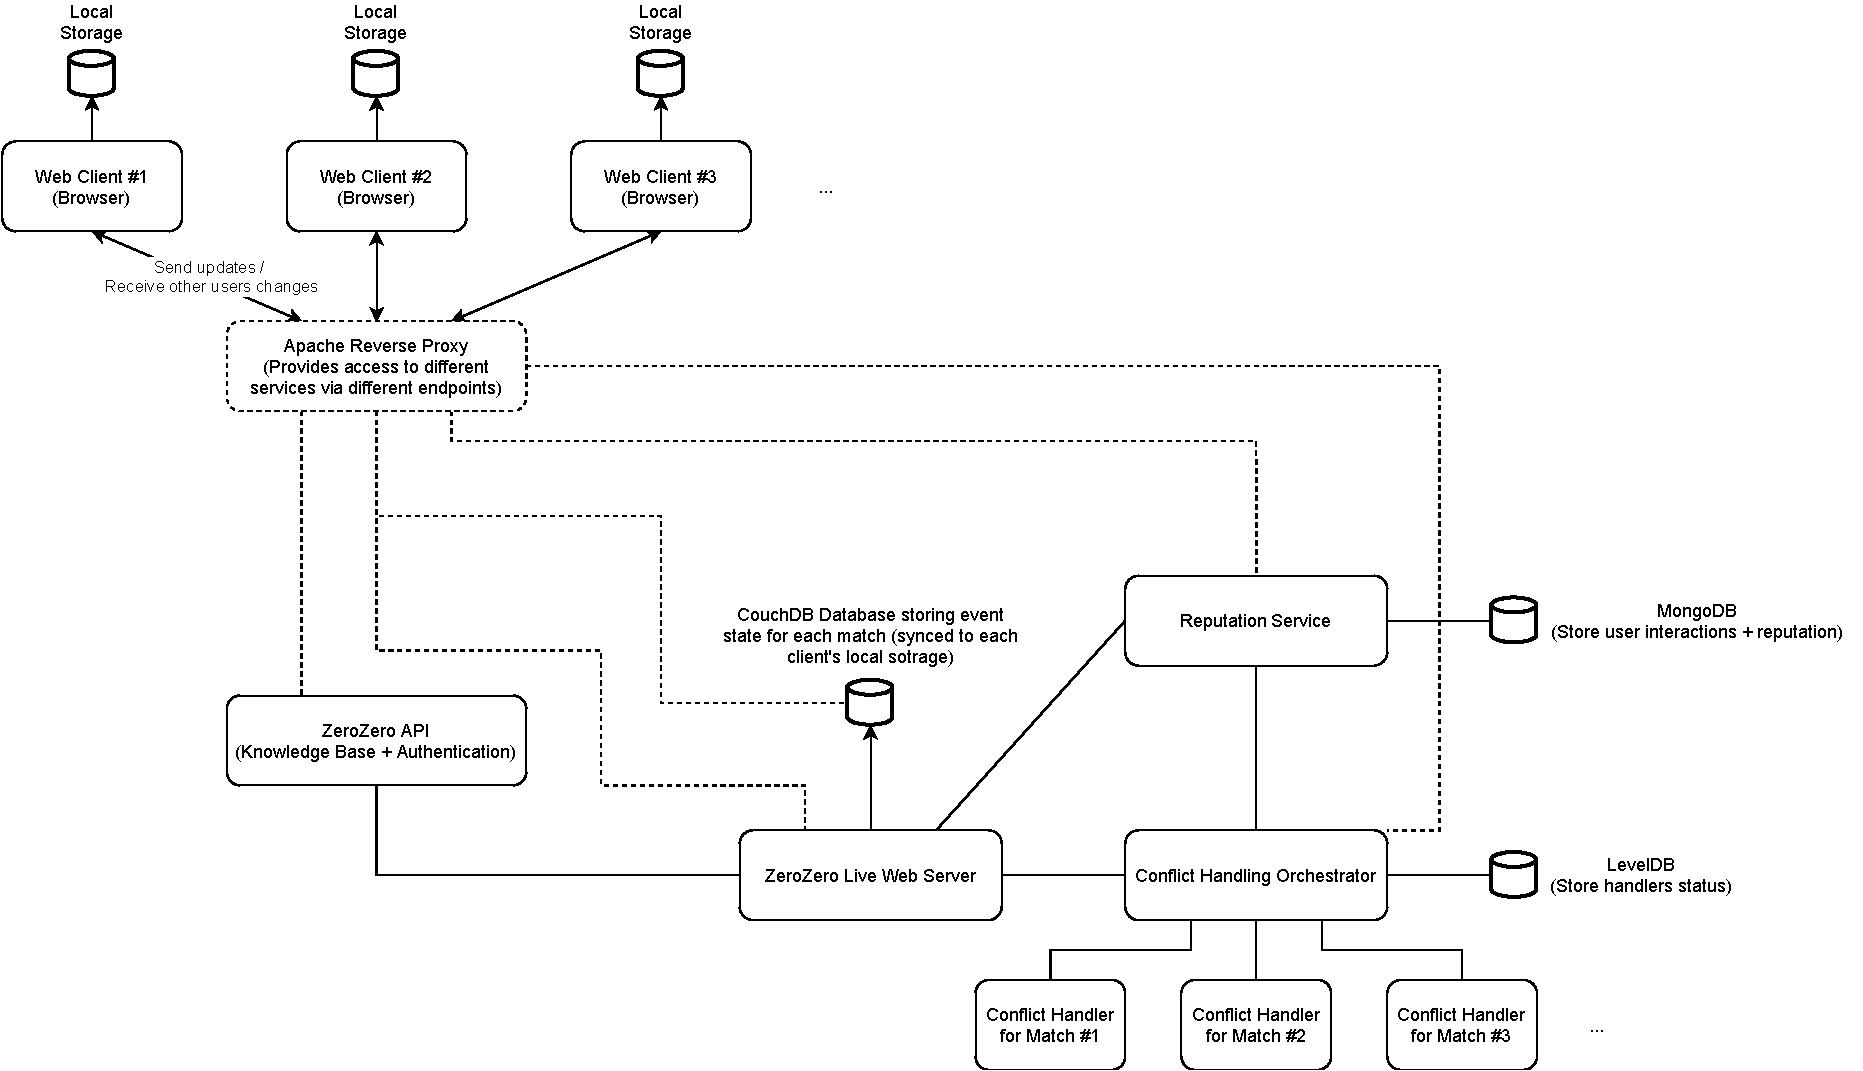
\includegraphics[width=\textwidth]{zerozerolive-arch.pdf}
        \caption{Architecture design of the zerozero.live system}
        \label{fig:services-arch}
    \end{center}
\end{figure}

\section{Reverse Proxy}

In the zerozero.live deployment, only the 443 --- HTTPS --- port is exposed to the internet, thus, to expose multiple services, it cannot be done in multiple ports, at least not from the outside. Due to this, a reverse proxy is required to map each service --- and its specific port --- to an endpoint on the main domain zerozero.live:
 
\begin{itemize}
    \item \textbf{/} Redirects to the client application --- the application's frontend;
    \item \textbf{/api} Redirects to a small proxy that communicates with the ZeroZero API;
    \item \textbf{/db} Redirects to the CouchDB, holding the match events in real time;
    \item \textbf{/manager} Redirects to the conflict handling services orchestrator, which monitors the conflict handlers for each match;
    \item \textbf{/reputation-manager} Redirects to the reputation service, which registers the interactions and calculates the reputation updates for users.
\end{itemize}

The following sections will dive deeper on the purpose and implementation details of each aforementioned service, which compose the whole application 

\section{CouchDB}

CouchDB is a document-oriented, multi-master database, which allows for easy replication between nodes. This enables data to flow seamlessly from web browsers to the database and vice versa, powering offline-first applications while being developer friendly, since the API that interacts with the local database --- powered by PouchDB --- is the same that interacts with the remote database --- CouchDB.

When compared to the previously analyzed alternatives, namely ShareDB and CRDT solutions such as Automerge, CouchDB is older and thus more \textit{battle tested} than the rest, while also having frequent releases --- the latest stable to date is from September, 2020. ShareDB has also been around for some time, since 2013, however, it offers a lower level alternative to conflict resolution using OT. It allows integration with any database and offers similar features to CouchDB, but I have found it difficult to program custom conflict resolution strategies, very much important to this work. From the three, Automerge is the youngest (2017), and it relies on a different approach to conflict resolution, based on CRDT. As it does not require a central server, it merges documents automatically and I could not find how to add custom resolution of conflicts, which led me to choose the CouchDB alternative.

It is based on documents which are JSON objects with at least an id and a revision identifier. CouchDB then uses this to detect conflicts --- if it has the same id, it may conflict --- and to resolve them. It works by creating a tree of documents, where the leaf nodes are the current winners, branches represent conflicting revisions, which are kept to be resolved by the application if needed. CouchDB will choose a winner automatically and deterministically, so that every client has the same version of the data. However it is possible to resolve the conflicts afterwards, by choosing a conflicting version as the winner, which appends a new node to the tree, after the previous winner, making the previously conflicting document the new leaf node, and thus the new winner for that document id.

Finally, this has the advantage of having a browser version, powered by PouchDB, which replicates the database to the browser's IndexedDB, and its API is the same as CouchDB's. This makes the application offline first, since all the changes are made to the local database, and continuously synchronized to the remote database.

\section{Conflict Handling}

Conflict handling is divided into two separate parts. One for the conflict handling of a single match, which is responsible to handle the conflicts themselves on the match level, and another for the orchestration of handlers themselves, which is responsible for the launching and orchestration of the match conflict handler processes. But first, it's important to set some concepts regarding conflict detection and documents' structure.

\subsection{Conflict Detection}

As events are introduced by users, conflicts may arise. The conflicting events are the ones whose documents share the same $\_id$. If we want documents to conflict, they cannot have unique ids, so the following structure was defined for each event $\_id$:
\begin{equation}
    eventMinute-eventMinuteExtra-eventCategory
\end{equation}

By having this structure, when any event from the same category is inserted, referring to the same game minute as another, they will conflict. Event categories are defined in such a way that events from different categories do not conflict. Some category examples include goal related events (\textit{Goal}, \textit{Own Goal}, \textit{Big Scoring Opportunity}, etc.), card related events (\textit{Yellow Card}, \textit{Red Card}), or time events (\textit{Start Whistle}, \textit{End of 1st Half}, \textit{Final Whistle}, etc.)

This will ensure that we have a basic conflict detection, however it can easily be noticed that even in the same category there may be events on the same minute: There can be a \textit{Big Scoring Opportunity} immediately followed by a \textit{Goal}, or even two \textit{Yellow Cards} for two different players, or even the same one which will wrongly conflict.

To improve the experience, a conflict handler is needed, in order to automatically solve conflicts as best as possible.

There are two concepts to understand going forward: events, and documents. Events are the instances of events, as used by the ZeroZero API, such as a \textit{Goal}, \textit{Own Goal}, or \textit{Big Scoring Opportunity}. These include the event type id, their category, some template text and a representative image to be rendered associated with it, among other fields. The complete list of events is present in Appendix~\ref{annex:api-events}. Documents are a wrapper on the API events, in order to be stored in the CouchDB database, and used on the ZeroZero Live exclusively. Their schema is defined in Table~\ref{table:document-schema}.

\begin{table}
    \centering
    \caption{CouchDB document schema}
    \begin{tabularx}{\textwidth}{|l|X|}
        \hline
        \textbf{Field}        & \textbf{Description} \\ \hline \hline
        \_id & the document id, used to detect conflicts, as explained above \\ \hline
        \_rev & the document's revision, in order to provide the history level of the changes tree of this document $\_id$ \\ \hline
        timestamp & a UNIX timestamp to help sorting the events that are generated for the same match minute \\ \hline
        id & the id of the corresponding event on the ZeroZero API, received on insert, and required to edit or delete this event from the API \\ \hline
        fk\_jogo & the match id \\ \hline
        equipa & the respective team's id \\ \hline
        fk\_user & id of the user that generated the event     \\ \hline
        fk\_jogador & id of the player the event refers to     \\ \hline
        fk\_jogador\_out & id of the secondary player the event refers to (used in the substitution event)     \\ \hline
        minuto & the match minute \\ \hline
        minuto\_extra & the extra minute, in case the event happened during injury time \\ \hline
        texto & the event's text (after template interpolation) \\ \hline
        event\_id & the event type id     \\ \hline
        fk\_live\_tpevent & the same as $event\_id$ \\ \hline
        ignore\_minuto & 1 if the minute should be ignored, 0 otherwise \\ \hline
        categoria & the event's category   \\ \hline
        vodafone\_clock\_time & a timestamp indicating the video mark when the event can be visualized \\ \hline
        insert & flag indicating if the event should be inserted to the ZeroZero\hyphenation{ZeroZero} API \\ \hline
        synced\_from\_api & flag indicating if this document came from a synchronization from the ZeroZero API, instead of being inserted by a user manually  \\ \hline
    \end{tabularx}
    \label{table:document-schema}
\end{table}

Regarding conflict resolution, the main fields to take into account are the $\_id$ and $\_rev$. A more detailed explanation is presented below on how these fields are used to detect and resolve conflicts between two documents.

\subsection{Conflict Handler}

As previously noted, the Conflict Handler will help resolve some existing conflict automatically, based on the conflicting events and the match context, in order to only rely on users to resolve pending conflicts as a last resource.

This is a Node.js process that will use PouchDB to connect to the remote CouchDB and listen for changes. It has two main responsibilities:
\begin{itemize}
    \item If the document does not have conflicts sync with ZeroZero API, by inserting, editing or deleting the event from their database, depending on the operation
    \item If the document has conflicts, try to resolve them according to the specified rules, by either deleting the conflict and keeping the current winner, deleting the conflict and adding it \textit{after} the previous winner, to choose it as winner, or keeping both documents, by deleting the conflict and adding a replicated document with a unique suffix added to the id so that it won't conflict again (See Figure~\ref{graph:keep-both-resolution}).
\end{itemize}

\begin{figure}[h]
    \centering
    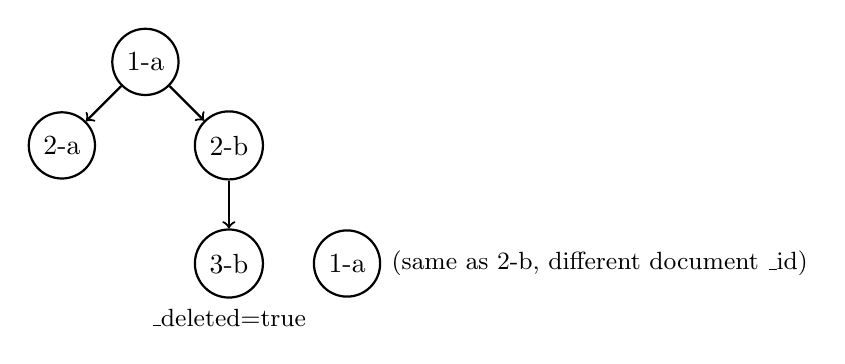
\begin{tikzpicture}[node distance={15mm}, thick, main/.style = {draw, circle}] 
      \node[main] (1) {1-a};
      \node[main] (2) [below left of=1] {2-a};
      \node[main] (3) [below right of=1] {2-b};
      \node[main, label=below:{\small \_deleted=true}] (4) [below of=3] {3-b};
      \node[main, label=right:{\small (same as 2-b, different document \_id)}] (5) [right of=4] {1-a};
      \draw[->] (1) -- (2);
      \draw[->] (1) -- (3);
      \draw[->] (3) -- (4);
  \end{tikzpicture} 
  \caption[Resolving a conflict by keeping both revisions]{Resolving a conflict by keeping both revisions --- \say{2-a} conflicts with \say{2-b} initially, then \say{2-b} is deleted, and a new document with a unique \_id is inserted (on the right), same as the deleted revision \say{2-b}}
  \label{graph:keep-both-resolution}
  \end{figure}

As it was mentioned earlier, all CouchDB documents have an $\_id$ and a $\_rev$ (as in \textit{revision}). When \textit{putting} a document --- CouchDB has a \textit{put} operation that allows insertions, edits and deletions, depending on the given argument --- if there is already an object with the same $\_id$, CouchDB will try to update it, however if the $\_rev$ does not match, a conflict is generated. For insertions, it only requires an object with at least an $\_id$ field. For edits, it requires the object with an $\_id$, referring to the document to be edited, and a $\_rev$, corresponding to the current revision of the document to be edited. For deletions, it requires the $\_id$, $\_rev$ and a $\_deleted$ field with a value of $true$, which is a special case of the edit operation. The deleted documents are not really removed from the database until a compaction operation\footnote{https://docs.couchdb.org/en/stable/maintenance/compaction.html} is performed to clean the deleted documents and older revisions are stripped, leaving only the necessary data required for conflict resolution operations.

Document revisions have two components: a number indicating their level in the tree of updates of that document, and a unique identifier. When a document is inserted, the generated revision starts with 1, and every time it updates, the successive revisions will have consecutive values e.g., 2, 3, and so on. This means that, considering two users are synchronized with the remote database which has a document with a revision of \say{1-xyz}, if they both want to update that document at the same time, they will both try to \textit{put} a document with \say{1-xyz} as its parent node. When CouchDB receives the requests, it will generate a revision for each, starting with 2, since their parent node revision starts with 1. One of them will be chosen as winner, and the other will conflict, since there are two documents on the same level: 2. The winner is automatically and deterministically chosen by CouchDB, so that every replica of the database is consistent, and it will store the conflicts for each document as well, then it's up to the application layer to resolve the conflict as needed. Figure~\ref{graph:couchdb-document-history} shows the history of a document's revisions, it starts on the revision level 1, then an edit generates the level 2 revision, and on the third level, there is a generated conflict, since two users tried to update it, by specifying the same root revision: \say{2-a}. CouchDB automatically chose revision \say{3-b} as the winner, but it still kept the \say{3-a} revision in memory. Figure~\ref{graph:couchdb-document-history-resolution} shows the same scenario, but adds the conflict resolution process, which works by deleting the revision we want to discard --- \say{3-b} in this case --- and since revision \say{3-a} becomes the only non-deleted leaf revision, it automatically becomes the winner and will be returned when someone fetches this document latest revision. The primary focus of this work starts here, by applying automatic conflict resolution strategies between the automatic CouchDB winner selection and the manual user conflict resolution that may happen afterwards.

\begin{figure}[h]
    \centering
    \begin{subfigure}[t]{.5\textwidth}
        \centering
        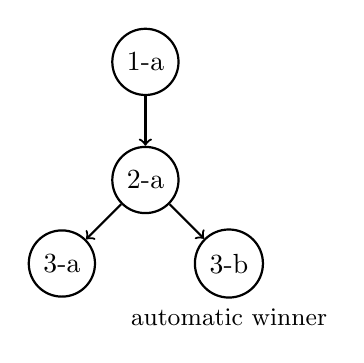
\begin{tikzpicture}[node distance={15mm}, thick, main/.style = {draw, circle}] 
            \node[main] (1) {1-a};
            \node[main] (2) [below of=1] {2-a};
            \node[main] (3) [below left of=2] {3-a};
            \node[main, label=below:{\small automatic winner}] (4) [below right of=2] {3-b};
            \draw[->] (1) -- (2);
            \draw[->] (2) -- (3);
            \draw[->] (2) -- (4);
        \end{tikzpicture} 
        \caption{Document revision history (conflict)}
        \label{graph:couchdb-document-history}
    \end{subfigure}%
    \begin{subfigure}[t]{.5\textwidth}
      \centering
      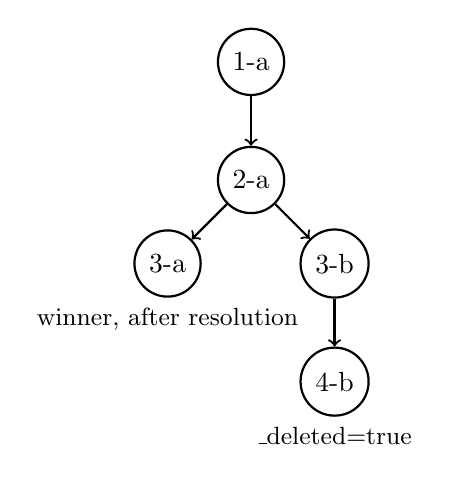
\begin{tikzpicture}[node distance={15mm}, thick, main/.style = {draw, circle}] 
        \node[main] (1) {1-a};
        \node[main] (2) [below of=1] {2-a};
        \node[main, label=below:{\small winner, after resolution}] (3) [below left of=2] {3-a};
        \node[main] (4) [below right of=2] {3-b};
        \node[main, label=below:{\small \_deleted=true}] (5) [below of=4] {4-b};
        \draw[->] (1) -- (2);
        \draw[->] (2) -- (3);
        \draw[->] (2) -- (4);
        \draw[->] (4) -- (5);
    \end{tikzpicture} 
    \caption{Document revision history (conflict) with conflict resolution}
    \label{graph:couchdb-document-history-resolution}
    \end{subfigure}
    \caption{Document revision history --- CouchDB model}
    \end{figure}

\subsection{Base conflict resolution strategies}

A base set of operations was defined in order to help solve conflicts. As per design, every conflict is resolved individually, i.e., if there are three documents conflicting, the conflict resolution will take place two times, one for each conflict pair (current winner, conflict). They all receive the pre-selected winner and conflict documents as arguments:
\begin{description}
    \item[\textbf{Leave Conflict}] This is the most basic resolution operation. It does nothing and leaves the conflict in the database, so that it can be resolved later in the frontend application;
    \item[\textbf{Ignore Conflict}] This is another basic resolution operation. It simply deletes the conflicting revision, basically agreeing with the automatic decision done by CouchDB;
    \item[\textbf{Choose a Winner}] This operation deletes the document passed as conflict and inserts a new revision as the winner;
    \item[\textbf{Keep Both}] This operation resolves conflicts by keeping both documents. Since there can't be two documents with the same id in CouchDB, otherwise they would conflict, it first deletes the conflicting revision, creates a new revision for the current winner, and inserts a new document equal to the conflicting one, but with a UUID\footnote{A UUID (Universally Unique Identifier) is a random 128-bit identifier. \cite{uuid-rfc}} appended to its default id. This ensures that it won't conflict with the existing document, however it has the downside that it won't conflict with anything ever again. While the initial document remains in the database, there will always be a \say{representative} of that set of ids, that will trigger conflicts every time a new document with that id is inserted. If that document is deleted, there is a workaround in place that selects a document from those with the same base id, and removes the random suffix, so that there is always some event to detect the conflicts for future inserts;
\end{description}

Additionally, there are specific resolutions that are triggered on the frontend --- not automatically ---- if the user resolves a conflict by choosing a winner or by keeping all conflicting documents:

\begin{description} \label{list:conflict-resolution-strategies-frontend}
    \item[\textbf{Choose One --- Frontend}] When choosing a winner, since there may be multiple conflicts at the same time, it needs to delete them all to fully resolve the conflict. However, if multiple users select different winners by each resolving the conflict differently, in the end they would end up deleting all documents. In order to avoid this, after deleting the loser documents, a new revision for the winner is inserted, so that if those multiple users select different winners locally, their choices will still conflict with each other after each \say{round} of conflict resolution. 
    \item[\textbf{Keep All}] This operation is similar to the \textit{Keep Both} operation in concept, but applied to $n$ documents at a time, not only 2 documents. It does so by first deleting all conflicts corresponding to a document id, then inserting new documents equal to the deleted conflicts, but with a UUID appended to the id, to make them unique, and avoid the conflict;
\end{description}

\subsubsection{Composite conflict resolution strategies}

By leveraging the aforementioned strategies, it's possible to create complex rules that apply to different event types that conflict with each other, provided that they happen in the same match minute and belong in the same event category.

\begin{description}
    \item[\textbf{Force Winner By Event Id}] Chooses as winner the document that has a given event id;
    \item[\textbf{Highly Conflicting; Ignore if same player}] If the player is the same, ignore conflict; Otherwise leaves the conflict intact to be resolved by the user;
    \item[\textbf{Goal vs. Own Goal}] In case a user reports a goal from team A, but another reports own goal from team B, they are both referring to the same goal, so the own goal event is chosen as winner, since it is more specific. Otherwise, leave the conflict to be resolved by the user;
    \item[\textbf{If same player, keep the one with given event id}] If the events refer to the same player, choose as winner the one that has the given event id; Otherwise leave the conflict to be resolved by the user;
    \item[\textbf{If different player, use reputation; Otherwise ignore}] If the referred players are different, choose as winner the event whose user has the highest reputation; Otherwise, ignore conflict;
    \item[\textbf{If same player, use reputation; Otherwise, keep both}] If the referred players are the same, choose as winner the event whose user has the highest reputation; Otherwise, keep both documents;
    \item[\textbf{If same player, ignore conflict; Otherwise, keep both}] If the referred players are the same, ignore the conflict; Otherwise, keep both documents;
    \item[\textbf{If same player, ignore conflict; Otherwise use reputation}] If the referred players are the same, ignore the conflict; Otherwise, choose as winner the event whose user has the highest reputation;
    \item[\textbf{Substitution Handler}] If the involved players are the same, ignore the conflict; If there are intersecting players, i.e., an event mentions player A out for player B, and the other event mentions player A out for player C, the conflict is left intact to be resolved by the user, later. Finally, if the involved players are different, keep both documents;
    \item[\textbf{Minute based resolution}] Receives a $minuteCondition$ function that takes the documents' minute as argument, a resolution function to execute if true, and a resolution function to execute if false. If $minuteCondition$ returns true, the first function is called, otherwise the second one is called;
    \item[\textbf{Choose biggest reputation}] Choose as winner the event whose user has the highest reputation;
\end{description}

\subsubsection{Synchronization with ZeroZero API} \label{sec:api-sync}

In order to fulfill User Stories \ref{user-story:sync-to-api} and \ref{user-story:sync-from-api}, specific logic was implemented to fetch missing events from the API, and to add them after consensus is reached on the ZeroZero Live platform i.e., there are no conflicts.

That being said, on the same loop that listens for changes and verifies if there are conflicts to resolve, the handler also two more branches of action: when the event is being synced from the API into CouchDB, and when the event has no conflicts and was not synced from the API.

Starting with the latter, the handler needs to know which operation was done regarding each event, in order to call the correct ZeroZero API. Each document comes as if we were receiving a CouchDB's \say{put} call, meaning that we don't know explicitly if it was an insert, edit or delete. In order to know if it is a delete operation, we can check for the $\_delete$ field. As was mentioned earlier, this field is true when the document is deleted. Regarding the distinction between inserts and edits, it's not as simple. On a first approach, revisions were used: if the revision level was 1, it was obviously an insert, otherwise it would be an edit to some existing document. This seemed rational, and it works to some extent, but not always. Recalling CouchDB delete behavior explained above, documents are not really deleted until the compaction operation is run. That means that if a document is deleted, another with the same id can be inserted afterwards, but since the first was not really erased from the database, the revision level of the newly inserted event will actually be different than 1, since the history for that document id is still there. In this case, this approach would consider some inserts as edits which would cause multiple events from being synchronized to the API correctly. In order to fix this, a special flag was added to each document, meaning if the document was meant to be inserted or not. On the client side, every event creation would generate a document with the $insert$ flag with a value of $true$. Whenever the handler inserted a document, it would edit it --- create a new revision --- setting the $insert$ flag back to $false$, so that it was not inserted every time there were changes to it. The final approach was then to check for the $insert$ flag in order to distinguish from insert and edit operations.

Regarding the synchronization from the ZeroZero API --- their internal storage of events, managed by the older platform, and used to show the match events on their website --- into ZeroZero Live, it's a bit more complex. First it shouldn't be continuous, or it would easily cause problems, since we would be adding events there and immediately receiving them back would probably cause some unwanted conflicts. With this in mind, every time there is a match page load --- on first visit, or on page refresh --- for every event that is on the ZeroZero API that has no correspondent document on CouchDB, there will be a synchronization attempt in order to add it to the CouchDB database. The reason because this is not as simple as inserting every event that is currently not in the ZeroZero live database yet, is because of potential conflicts: Events that are already on the ZeroZero side, should not conflict with each other, and they also should not conflict with CouchDB documents, on the synchronization phase, at least.

First, let's explain how events are known to be synchronized or not. Every time there is an insert of a document on ZeroZero Live, and it is synchronized \textit{to} the ZeroZero API --- as per the logic described above --- the API returns an id for that event, that is different from the document's $\_id$. That id is used identify the event on the ZeroZero side, allowing us to call the edit and delete APIs on the events. When the CouchDB document is synchronized to the ZeroZero API --- the insert API is called ---, the document is edited to set the $insert$ flag to false, as mentioned above, but it also sets the $id$ field, meaning that the document has a ZeroZero's event counterpart.

Based on this, for every event coming from the ZeroZero API, we can check if there is a CouchDB document with a corresponding $id$, if there isn't, that event needs to be inserted into CouchDB.

For those that need to be synchronized, they are inserted as normal documents, as if they were inserted by the user, however, the document $\_id$ has an appended \say{synced\_from\_api} suffix, so that the handler will know to use the synchronization algorithm, instead of simply inserting the event.

\begin{figure}[h]
    \begin{center}
        \leavevmode
        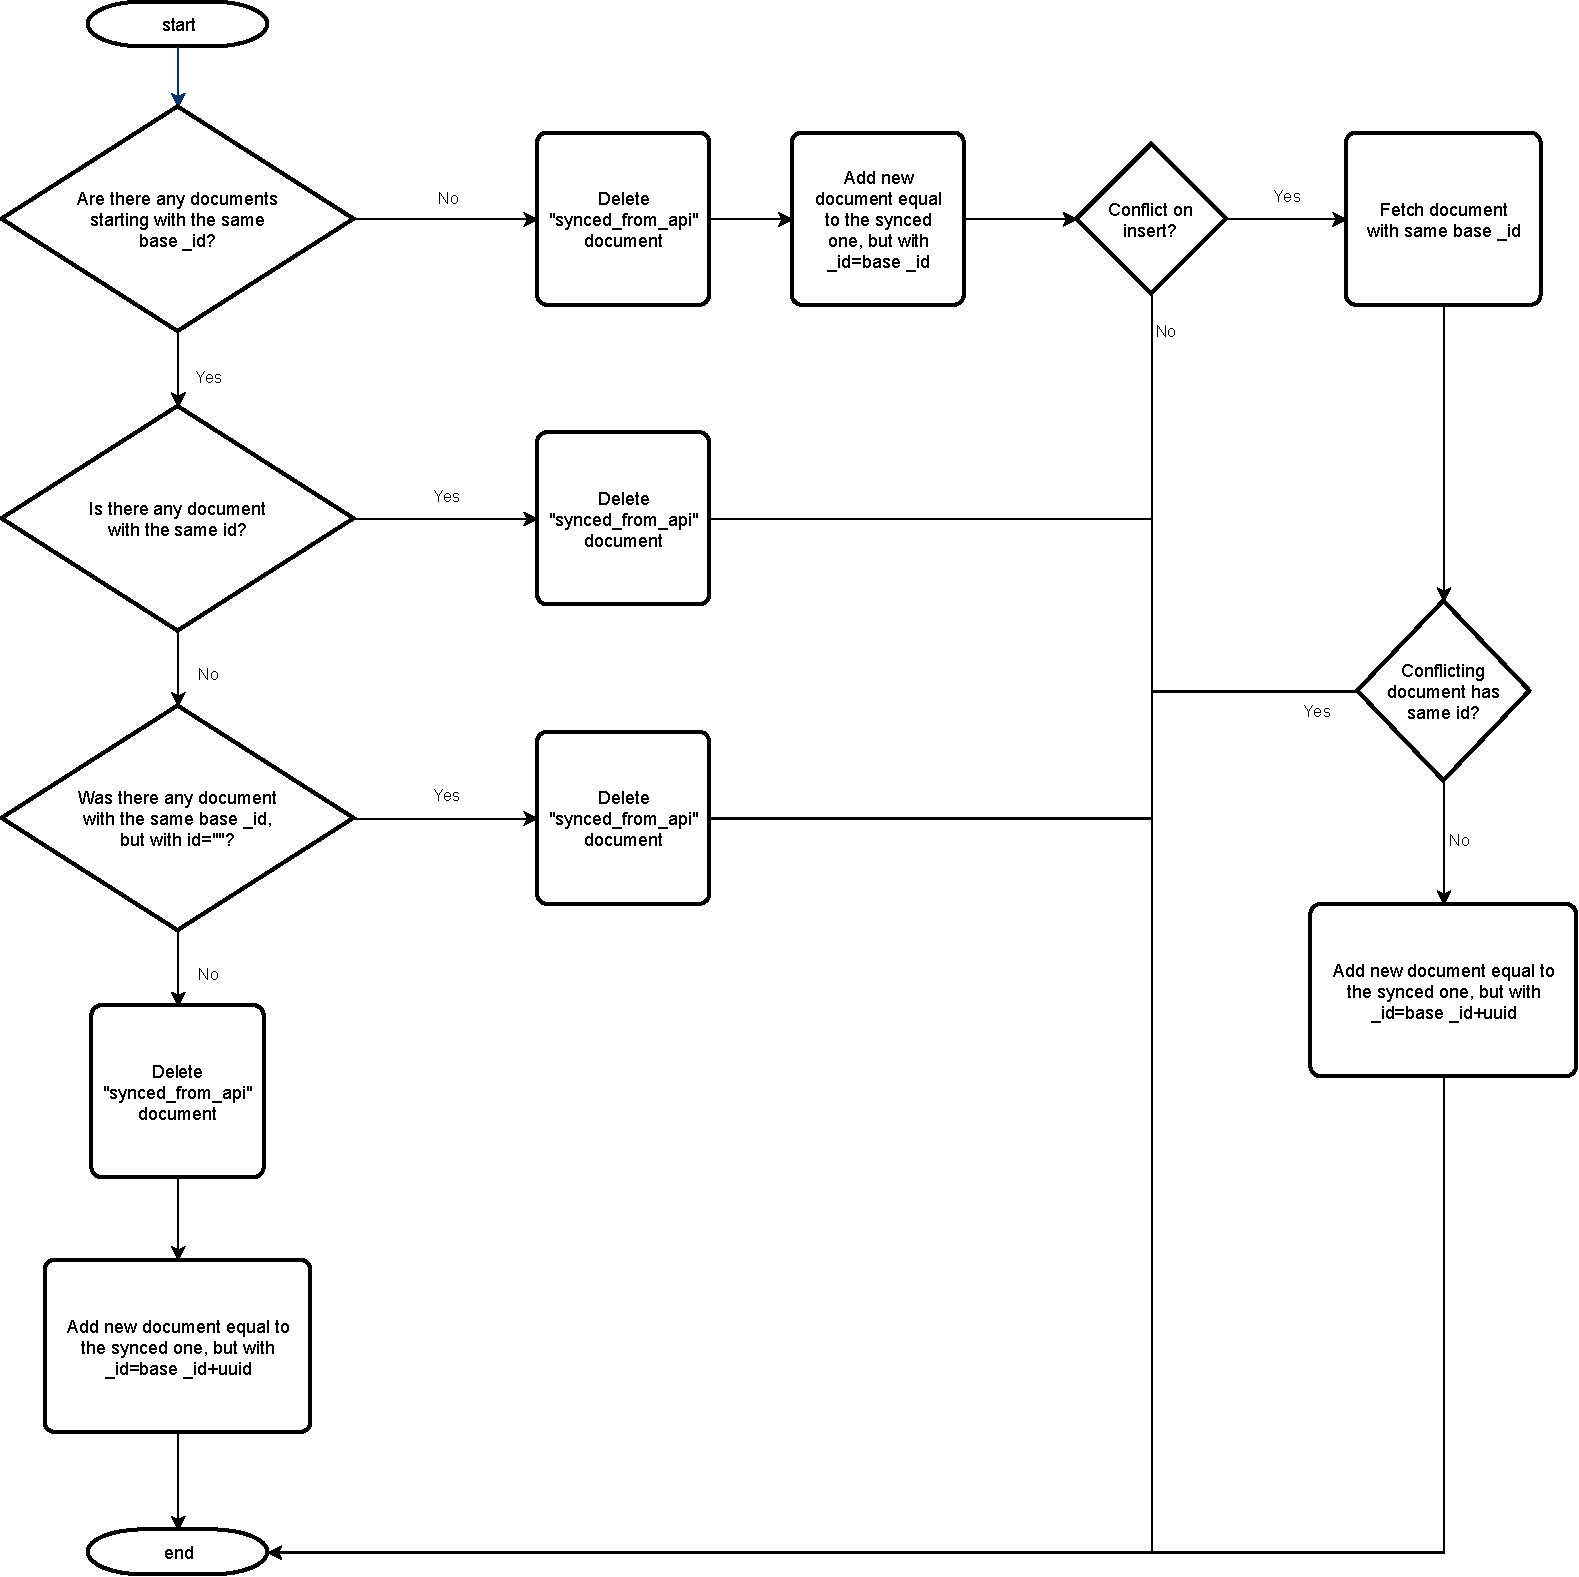
\includegraphics[width=\textwidth]{sync-api-flow.pdf}
        \caption{Synchronization of events from ZeroZero API into ZeroZero Live database}
        \label{fig:sync-from-api-flux}
    \end{center}
\end{figure}

Figure \ref{fig:sync-from-api-flux} shows the flowchart relative to the algorithm of synchronization of events into CouchDB. It first checks if there are documents starting with the same base $\_id$. The base $\_id$ is the $eventMinute-eventMinuteExtra-eventCategory$ string used to identify documents and allow for conflict detection. Due to custom resolutions like \textit{Keep Both} or specific document types that never conflict --- such as comments --- some documents will have a base $\_id$ followed by a unique part, in UUID format, thus it's important that it is ignored, otherwise some events would never be caught by the synchronization algorithm. It's also important to note that even if there is a document with a same base $\_id$, they may not refer to the same event, and not even correspond to the same event type, it just means they happened at the same minute, and belong to the same event category. The only way there is to know if a synchronization candidate --- i.e., the one with \say{synced\_from\_api} appended to the $\_id$ ---  is the same as an existing document, is by comparing their $id$s, not $\_id$s, as that value comes from the ZeroZero API.

First, if there are no documents in the CouchDB database that have a same base id, we can know for sure that that event is not in the CouchDB database yet, thus, the \say{synced} document is deleted, and a clone is inserted with the correct $\_id$ --- i.e., the base $\_id$ --- so that it can conflict in the future with other events. However, imagine that while this is happening, someone inserts an event at the same minute with the same category. That will prevent us from inserting the new version of the \say{synced} document, so there is a check in place that verifies the conflicting document and if it has the same id, the algorithm stops, since the event is already there, otherwise, it will add it, but with a unique UUID suffix, so as to avoid the conflict on insertion.

If there are any documents with the same base $\_id$, however, it will try to find out if among those there is some that has the same id. If so, it will simply delete the \say{synced} document, it is already synchronized. If not, and if among the searched documents there's some that have an empty id --- meaning they are in the middle of the process of getting one, after the insert call --- the algorithm will delete the \say{synced} document as a preemptive measure, hoping it will be there in the future. The next time this algorithm runs, that document will already have an id, and the check above can be done.

Finally, if there were documents with the same base $\_id$, but none had the same id nor had empty ids, the synchronization candidate is not present, but must be added with an unique suffix, to prevent insertion conflict.

\subsection{Conflict Handling Orchestrator}

In order to have multiple handlers at once, which is needed as there may be multiple matches happening at the same time, one needs to have a controller that handles their initialization, manages their status and stops them once they are not needed anymore.

That is the responsibility of the Conflict Handling Orchestrator. It is a simple Node.js application that exposes an HTTP API, that lets us initialize a conflict handler for a given match, list active handlers, stop a conflict handler for a given match, and \textit{kill} any \textit{zombie} handler references that might be left over after a crash. The state of the handlers is kept in a LevelDB\footnote{https://github.com/google/leveldb} database, which is a simple key-value database. Each record will have the match id as the key and the value is an object containing the PID of the handler process for that match, as well as the timestamp of when the handler was started.

Even though the orchestrator is the parent process of the conflict handlers, in case the conflict handler process fails, the orchestrator is independent enough that it won't terminate as well. If the orchestrator itself fails for some reason, it is built to auto-restart instead of making the docker container restart, which would make it lose context and terminate all other processes, including child conflict handlers. This is why information about the handlers is kept in a separate database, instead of in-process memory, so that the orchestrator can recover all of it in case of failure.

\paragraph{POST /initConflictHandler/:matchId}
This endpoint launches a child process running a conflict handler for the specified match, as described in the previous subsection. It is made in such a way that it won't allow the launch of multiple handlers for the same match simultaneously. After a specified timeout, the child process is killed, to avoid wasting resources on finished matches.

\paragraph{POST /stopConflictHandler/:matchId}
This endpoint terminates a process associated with the given match.

\paragraph{GET /active-handlers}
This endpoint returns a list of active match conflict handlers, together with their respective PIDs.

\paragraph{POST /cleanup-zombies}
This endpoint will verify that every stored match handler is actually running. If not, it will update the database. This is important because after some failure, conflict handlers might not be running as the database shows, and this endpoint will restore the truth.

\section{Reputation Service}

In order to aid the automatic conflict resolution, in many cases, the reputation of the users will be used to determine which event to choose as the conflict winner. This is only done for conflicts that are not critical. For any important conflict --- such as \textit{Goal from team A} vs. \textit{Goal from team B} --- it is left for users to resolve manually on the UI.

The Reputation System is based on the fact that people that input conflicting events disagree with each other, as well as who edits or deletes an event. Every time a user receives an event from someone, they implicitly agree with it, until they act to mark disagreement, executing any of the actions described before. Finally, users can explicitly agree with each other, by inputting conflicting events, that are exactly the same i.e., if two users report a goal from team A at the same time, they are not disagreeing with each other, but rather agreeing. This is considered a more \textit{powerful} agreement, since they both explicitly inputted the event, instead of just waiting for someone to do it and passively reading it. These are the three interaction types that are registered by the reputation service.

The Reputation Service is a Node.js microservice that exposes an HTTP API, and uses a \mbox{MongoDB} database to persistently store data. It has endpoints to register interactions between users and inputs and another endpoint to calculate reputation updates after a specific match interactions. MongoDB was chosen due to its good horizontal scaling ability, which is useful for future-proofing the application, without losing too much performance currently. Additionally, there's a lack of relationships between the collections, thus an SQL-based alternative is not necessary.

The database will store the interactions, which are documents containing the $matchId$, $eventId$, $userId$, $eventOwnerId$, $isProcessed$ and $interactionType$ fields. $matchId$, $eventId$, and $userId$ uniquely identify an interaction and are used to prevent the same user from registering multiple interactions for the same event. Additionally, there are checks in place so that a user cannot register interactions for an event they have inserted. $isProcessed$ is a boolean flag that marks the interaction as processed by the reputation calculation, so that it is not used multiple times when calculating reputation updates. Finally, the $interactionType$ defines the type of interaction, which affects the reputation update calculation, e.g., $Agree$, $Disagree$, $Explicit Agree$

Additionally, the database has another collection to store the user and their respective reputations, to be used in the conflict resolution. Each document has $userId$, $reputation$ and $updatedAt$ fields. The $reputation$ represents the numerical value of the reputation of the user with id $userId$, and the $updatedAt$ field is used to calculate the reputation decay --- the more time passes after the previous reputation calculation, the more its reputation will decay due to inactivity.

\paragraph{GET /:userId/reputation}

This endpoint returns the current reputation for the given user.

\paragraph{POST /:matchId/:eventId/:eventOwnerId/:userId/agree}

This endpoint is called every time a user receives an event in their local database. It means that they \textit{implicitly} agree with that input, since they haven't yet done something else to manifest any intention on the contrary. Like the other interactions, it does not allow self-voting, and is overwritable, meaning of course that once a user wants to disagree with some input, the previous implicit agreement will be nullified. Finally, it cannot overwrite any existing interaction on the same input, since this endpoint is made to be called automatically, it can be done without worrying about overwriting any other explicit interactions.

\paragraph{POST /:matchId/:eventId/:eventOwnerId/:userId/disagree}

This endpoint is called every time a user edits or deletes an event, or when there is a conflict. It means that the user \textit{implicitly} explicitly disagrees with that input, since they have done something to manifest any intention. Like the other interactions, it does not allow self-voting, but it is not overwritable, meaning that once a user disagrees with some input, that disagreement is forever. Finally, it can overwrite any existing interaction on the same input, since this endpoint is made to be called explicitly, after any automatic interactions may have been recorded.

\paragraph{POST /:matchId/:eventId/:eventOwnerId/:userId/explicit-agree}

This endpoint is called every time a user inserts and event that conflicts with another event that is essentially the same. It means that, even though the events conflict, they are the same, so both users are explicitly agreeing with each other. Like the other interactions, it does not allow self-voting, but it is not overwritable, meaning that once a user explicitly agrees with some input, that agreement is forever. Finally, it can overwrite any existing interaction on the same input, since this endpoint is made to be called explicitly, after any automatic interactions may have been recorded.

\paragraph{POST /:matchId/updateRep}

This endpoint calculates and updates the reputation of the users involved in a specific match. It runs the reputation algorithm that uses the stored interactions to calculate a new reputation for each user. The algorithm is based on the ideas presented in Section~\ref{sec:rep-sys-sota}, as it takes into account the different types of interactions as well as a reputation decay over time.

First, for every user involved in the match, it will calculate a reputation decay multiplier based on the last time the reputation was calculated for that user --- users that stay inactive for longer get a bigger penalty. 

\begin{equation}
    newUserRep = oldUserRep * decayCoefficient^{timeSinceLastUpdate}
\end{equation}

Then, for every recorded interaction, it will calculate the set of deltas that corresponds to the effect of a specific interaction on a specific input. Different interactions result in different deltas.

For agreements:
\begin{equation}
    deltaA = baseInputRep * maxRepReward * userRep * userRepInfluence
\end{equation}

For disagreements:
\begin{equation}
    deltaD = -baseInputRep * (1 - (maxRepReward * userRep * userRepInfluence))
\end{equation}

For explicit agreements:
\begin{equation}
    deltaEA = (deltaAgreement) * (1 + explicitAgreementBonus)
\end{equation}

After calculating all the deltas for each interaction, they are marked as processed, to avoid being used mutiple times when calculating reputation updates. Users' reputations are then updated according to the average of the deltas of their concerning interactions:

\begin{equation}
    repIncrement = (1 - userRep) * avgDeltas;
\end{equation}

\begin{table}
    \centering
    \caption{Reputation service constant values}
    \begin{tabular}{|l|l|l|l|}
        \hline
        \textbf{Constant}                   & \textbf{Value} \\ \hline \hline
        Initial User Reputation             & 0.2 \\ \hline
        Base Input Reputation               & 0.01    \\ \hline
        Maximum Input Reputation Reward     & 0.05    \\ \hline
        Maximum Input Reputation Punishment & 0.1    \\ \hline
        User Reputation Influence           & 0.2    \\ \hline
        Explicit Agreement Bonus            & 0.2    \\ \hline
        Reputation Decay Coefficient        & 0.85    \\ \hline
    \end{tabular}
    \label{table:reputation-constants}
\end{table}

The used constant values are defined in Table~\ref{table:reputation-constants}. With this configuration, it takes approximately one month --- 4 weeks --- for a user to lose half of their reputation.

\section{Web Application (Frontend)}

The last component, and arguably the most important --- How would users use the application otherwise? --- is the frontend web application. For browsers, it's a set of HTML, CSS and JavaScript files being served by an Nginx web server. Many web applications have this setup, but let us dive deeper on the process that happens before the generation of those files to be served.

The application is built with React and is essentially a \textit{Single Page Application} (SPA), but regardless of the nomenclature, the application provides multiple interfaces, or pages. It doesn't work like the usual multi-page web application, since there is indeed only one page being served --- index.html --- however, the JavaScript, namely the React Router package, handles the routing and the URLs, by rendering different component trees based on the URL, and thus emulating a multi-page setup.

The majority of the frontend application was already built before. Figures~\ref{fig:zerozerolive-login}, \ref{fig:zerozerolive-home}, \ref{fig:zerozerolive-search}, \ref{fig:zerozerolive-history} represent interfaces that were mostly untouched during the development of this work, as they are of no interest to the real-time multi-user collaboration problem this work addresses. Figure~\ref{fig:zerozerolive-teams} shows the interface to pick the roster of each team. There were no major changes to it apart from fixing an issue where users could not change pages too fast, as it might not submit their information correctly.

\begin{figure}[h]
    \begin{center}
        \leavevmode
        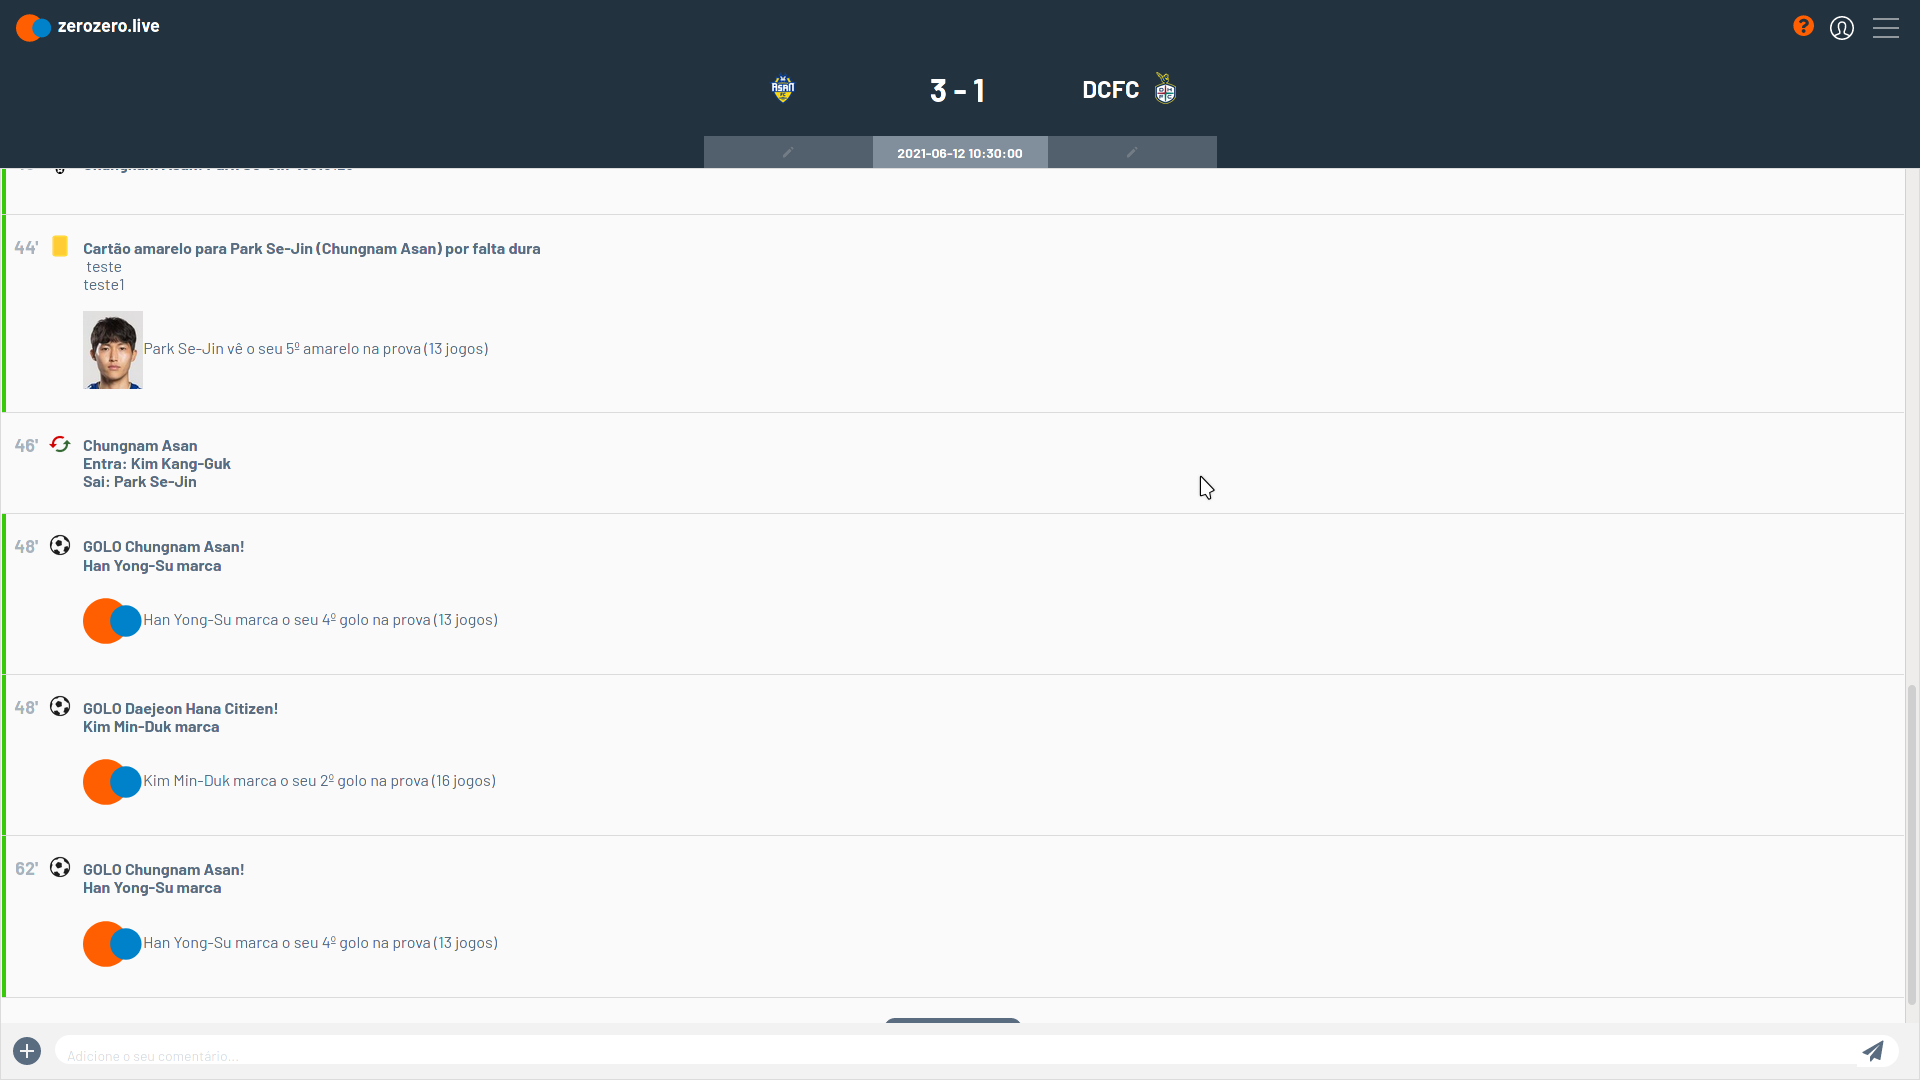
\includegraphics[width=\textwidth]{zerozerolive-comments.png}
        \caption{Comments page for a match in zerozero.live}
        \label{fig:zerozerolive-comments}
    \end{center}
\end{figure}

\begin{figure}[h]
    \begin{center}
        \leavevmode
        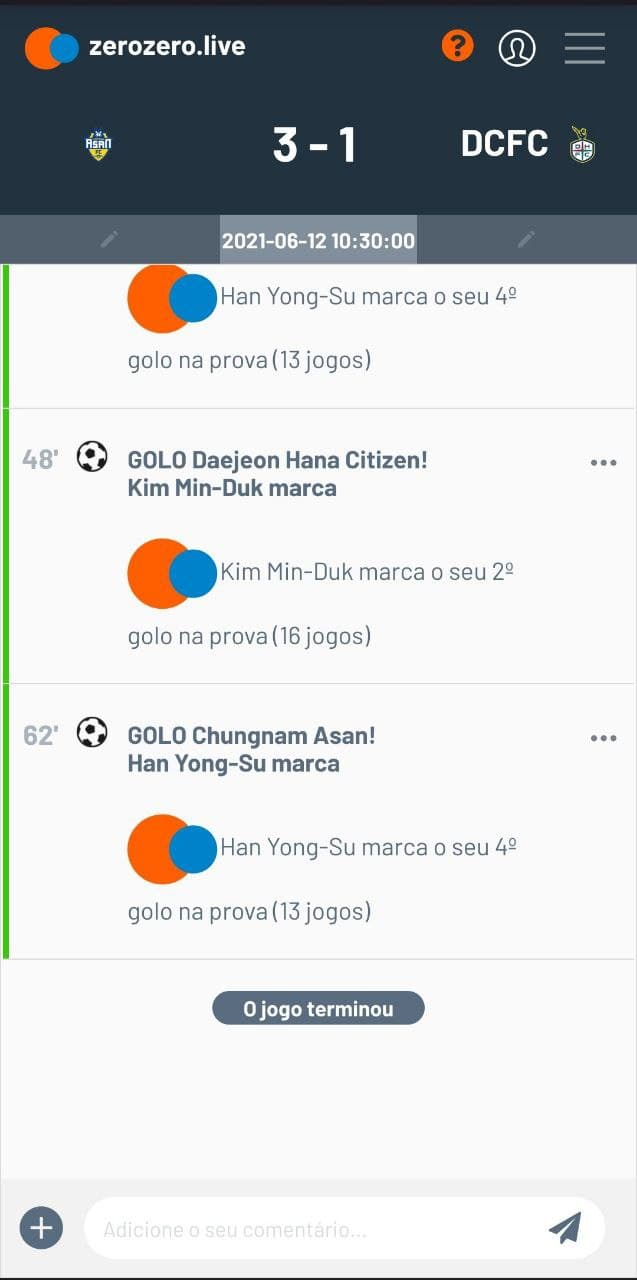
\includegraphics[width=0.3\textwidth]{zerozerolive-comments-mobile.jpg}
        \caption{Comments page for a match in zerozero.live --- Mobile version}
        \label{fig:zerozerolive-comments-mobile}
    \end{center}
\end{figure}

Figures~\ref{fig:zerozerolive-comments} and \ref{fig:zerozerolive-comments-mobile}, desktop and mobile interfaces, respectively, represent the page where most of the work was focused: the match commentary. It feature the match information on top, the events list at the middle, as well as the input area on the bottom. It purposefully resembles a chat application, so that it is intuitive for users how to use the application.

It executes some operations in order to present the events to the user. First, it initializes a local PouchDB database, or connects to it if it already exists, and does the same with the remote CouchDB database, except that it doesn't try to create it if it doesn't exist, that is a responsibility of the respective conflict handler. After connecting to both databases, it loads any existing events on the local database to the UI, to promote the offline-first behavior. The user will always see anything the already have locally first. Then it starts the replication listener, in order to listen for remote changes and replicate those to the local database, so that the user can get the remote updates and see the other events on their timeline.

Then, it tries to sync any pending information that is stored locally to the remote database, which may happen when the connection is lost.

At the same time, it will load the match information from the ZeroZero API, including the selected rosters, available event types, score, match time and state and substituted players. This is important in order to load the players correctly when choosing the player for the inputted event. This information is refreshed every 30 seconds.

\begin{figure}
    \centering
    \begin{subfigure}[t]{.5\textwidth}
        \centering
        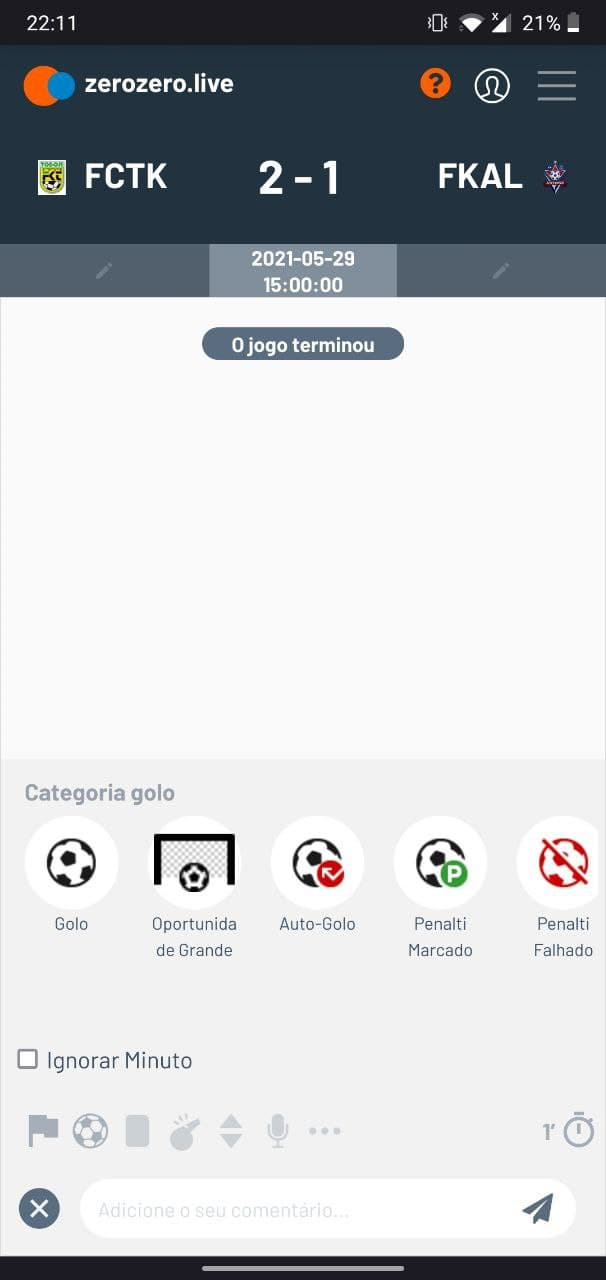
\includegraphics[width=0.8\textwidth]{zerozerolive-event-select.jpg}
        \caption{Event selection}
        \label{fig:zerozerolive-event-select}
    \end{subfigure}%
    \begin{subfigure}[t]{.5\textwidth}
        \centering
        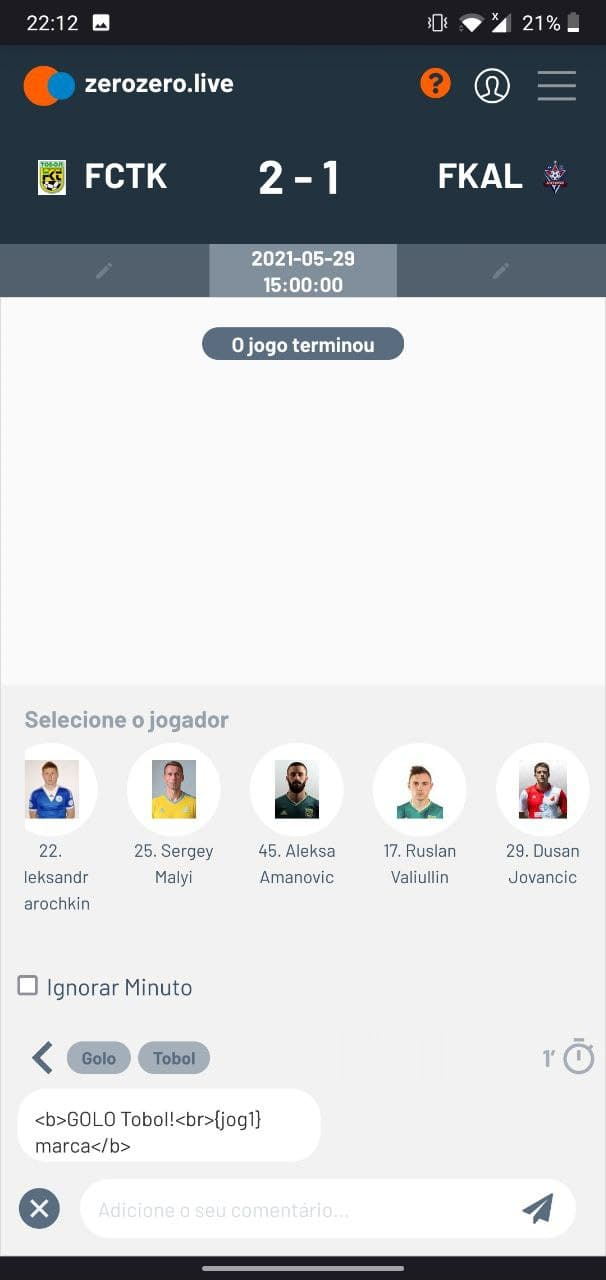
\includegraphics[width=0.8\textwidth]{zerozerolive-event-player-select.jpg}
        \caption{Event's player selection}
        \label{fig:zerozerolive-event-player-select}
    \end{subfigure}
    \caption{ZeroZero Live --- Input interface}
\end{figure}

As was previously mentioned, a big part of this project is the synchronization with the ZeroZero API events. On startup, the application will check which event are on the API registry that are currently not on the ZeroZero Live database. If it finds any, it will try to synchronize them by inserting them in the local PouchDB database, and then replicating to the remote database. The complete algorithm is mentioned in more detail above, on Section~\ref{sec:api-sync}. 

%events interactions(insert, edit delete) (to local then remote)
Regarding the event operations, namely insert, edit, and delete, the process is similar to each of them. A document is pushed to the local database, which makes it show on the UI for the user. Then it is synchronized to the remote database which, due to the replication listener will make it show on other users' machines as well, as soon as it replicates to their local databases. It may happen that during these replications a conflict arises. In those cases, the conflict icon is shown on the event (see Figure~\ref{fig:zerozerolive-conflict-event}), and the user can resolve the conflict after clicking there and examining the solution candidates. Figure~\ref{fig:zerozerolive-conflict-resolution} shows the conflict resolution interface, where the user can select a \say{winner} event, or choose to keep all events in the match. The resolutions strategies were already discussed above, in Section~\ref{list:conflict-resolution-strategies-frontend}

\begin{figure}
    \centering
    \begin{subfigure}[t]{.5\textwidth}
        \centering
        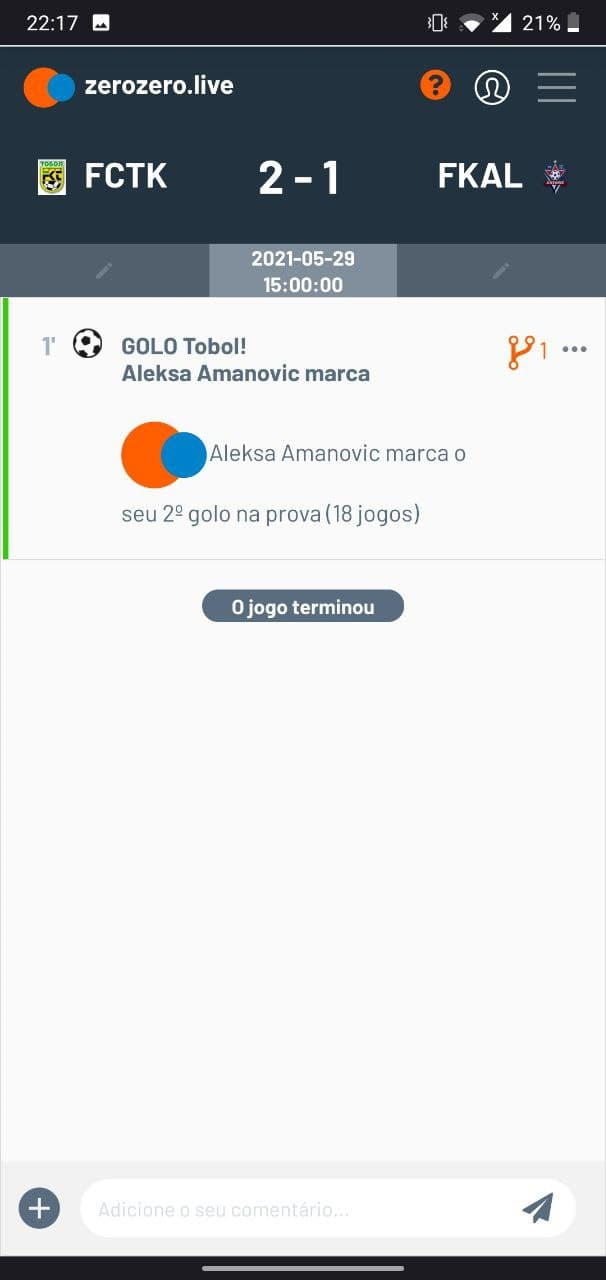
\includegraphics[width=0.8\textwidth]{zerozerolive-conflict-event.jpg}
        \caption{Event with a conflict pending resolution}
        \label{fig:zerozerolive-conflict-event}
    \end{subfigure}%
    \begin{subfigure}[t]{.5\textwidth}
        \centering
        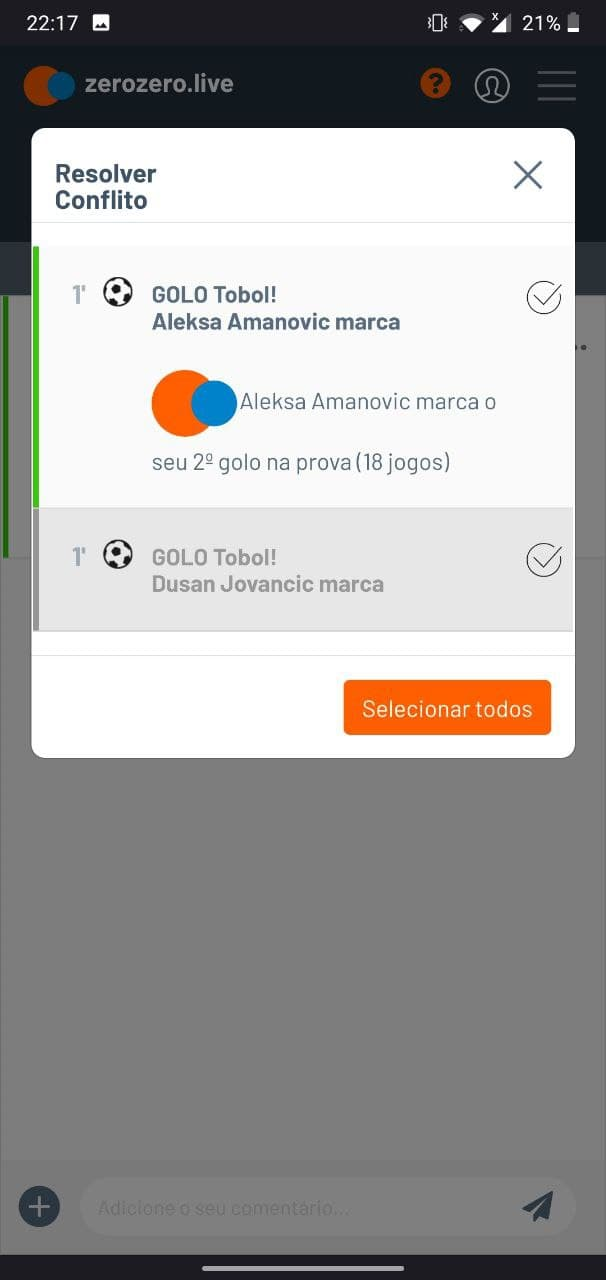
\includegraphics[width=0.8\textwidth]{zerozerolive-conflict-resolution.jpg}
        \caption{Event conflict resolution interface}
        \label{fig:zerozerolive-conflict-resolution}
    \end{subfigure}
    \caption{ZeroZero Live --- Conflicts interface}
\end{figure}

Figure~\ref{fig:insert_doc_seq_noconf} shows the sequence of operations when an event is inserted on the frontend (Browser), when there is no conflict. First the document is created on the local database, which is then replicated to the remote database. Once the remote database receives a document, it will emit events for any listener, including the clients and the conflict handler which, when receiving a document without conflicts, will try to synchronize it to the ZeroZero API, by inserting it in this case. As was previously mentioned, it will then update the document by setting its \say{insert} field to $false$. That change will once again be propagated to all listening clients.

In the case of conflicts, Figure~\ref{fig:insert_doc_seq_conf} shows that the sequence of operations is slightly different when the conflict handler receives the conflicting document. It will resolve it first, before trying to synchronize anything. One thing to note is that the UI will receive the conflicting event while it is being resolved. For the users, it is as if someone is resolving a conflict really fast, as they might see the conflict appear and quickly be resolved, since the changes are always replicated to all listening clients. After resolving the conflict and receiving the updated document back, the conflict handler will behave like the previous example and synchronize the documents accordingly.

\begin{figure}[h]
    \begin{center}
        \leavevmode
        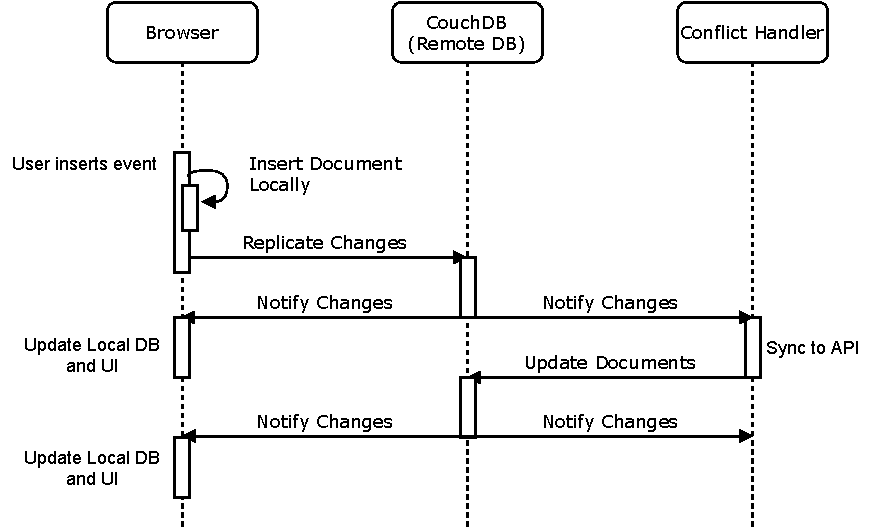
\includegraphics[width=\textwidth]{insert_doc_seq_noconf.pdf}
        \caption{Sequence diagram representing the flow when inserting an event without conflicts}
        \label{fig:insert_doc_seq_noconf}
    \end{center}
\end{figure}

\begin{figure}[h]
    \begin{center}
        \leavevmode
        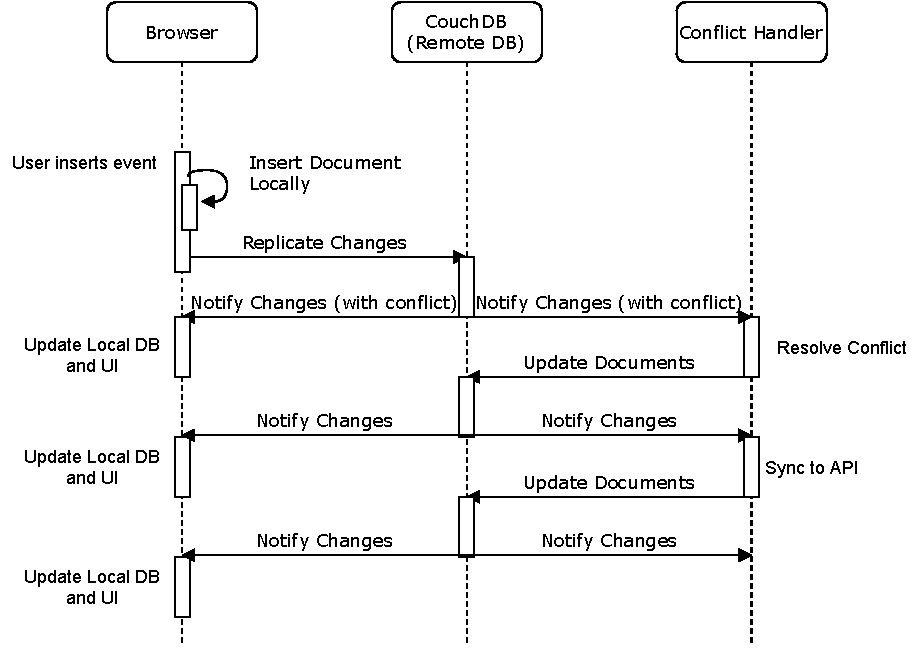
\includegraphics[width=\textwidth]{insert_doc_seq_conf.pdf}
        \caption{Sequence diagram representing the flow when inserting an event with conflicts}
        \label{fig:insert_doc_seq_conf}
    \end{center}
\end{figure}

\section{Time synchronization}

An important part of a real-time application is the time synchronization between users and the server itself. In this application this is done by clients fetching the game start time from the ZeroZero API, and calculating the game time locally. It has a big problem, as we eventually found out, since clients may not be synchronized with the server themselves. A similar scenario happened inside ZOS, while we were testing the application. Some of the computers in the office had their clocks offset by a couple minutes in relation to the server serving the application. This resulted in a shift on the match minute they were seeing. This happened since the match clock is calculated based on the start time specified on the server and the current client time. In order to fix this problem, and any similar issues that can happen for users in different timezones, an offset correction value was added. The clients now send their local time when requesting the match information, and the server will return an offset in relation to its own time, which clients can use to fix the clock calculation, and make sure all are synchronized, independently of their local times.

\section{Summary}
In summary, a microservice architecture was used to build the application to solve the problem defined in Chapter~\ref{chap:problem}. In order to organize the deployment and treat the whole system as a unit instead of managing all the microservices individually, Docker Compose was used. In order to allow multiple services to be reached through the same domain, a reverse proxy service was developed, which routed the requests to the different services based on the used endpoint. In order to deal with conflicts detection and resolution, CouchDB was used, which has these features built-in to its design, while allowing an easy replication and offline usage, by using its local counterpart, PouchDB. Additionally, a reputation HTTP server was developed to handle the user reputation, which takes into account the users' reputations in order to have a dynamic influence on each others' inputs, as well as a decay of reputation over time, if users become inactive. All of these features were visible to the user through the web application frontend, which allowed for match coverage, by selecting the teams' rosters and events inputting, describing what is happening in real time. It further allows for manual conflict resolution when the automatic resolver chooses not to resolve the conflict.
\chapter{Evaluation and Analysis}\label{chap:evaluation-and-analysis}


There are two types of target users in this platform. The first are the current ZeroZero's sports journalists who cover matches professionally, and have a platform where they do that already. They rely on it to update the match details on the ZeroZero platform. The second are casual people who like to follow lower division matches, due to the lack of coverage. With this in mind, different experiments were made, depending on the type of users and their use cases.

\section{Experiments Monitoring}

In order to better understand how the user is interacting with the application and pinpoint some aspects that might be worth improving, we intend to measure some aspects of the interaction. Next are some proposed metrics, which are relevant to this study. They are divided on their type for clearer understanding.

\begin{enumerate}
    \item Performance metrics:
    \begin{enumerate}
        \item Number of automatically-unsolved conflicts during an event per user
        \item Number of total generated conflicts
    \end{enumerate}
    \item Self-Reported metrics, asked in the form of a Likert scale\footnote{A typical item in a Likert scale is a statement to which respondents rate
    their level of agreement. The statement may be positive (e.g.,\ “The terminology used in this interface is clear”) or negative (e.g., “I found the navigation options confusing”). Usually a five-point scale of agreement like the following is used: 1. Strongly disagree 2. Disagree 3. Neither agree nor disagree 4. Agree 5. Strongly agree}, when appropriate:
    \begin{enumerate}
        \item The tool allowed the user to narrate the game without issues
        \item The user considered the number of conflicts... (1 - low; 5 - high)
        \item The user believed the events to correspond to the match's truth 
        \item The conflicts were easily to locate
        \item The conflicts were easy to solve \\
        \item The user has used another mean of communication with friends while following the match in order to discuss it (*) 
        \item The user would use the tool again in the future (*) \\
        \item Open answer to allow users to give whatever feedback they might have
    \end{enumerate}
\end{enumerate}

(*) Yes or No questions

\section{The Journalist Use-Case}
% often works alone, relies on the correct api sync (uses a more broad set of events)
% constant feddback-deployment loop
When covering a match, journalists usually work alone, as they are assigned different matches to cover. As such, they rarely face conflicts, but they also rely on the API syncronization feature heavily, as it is literally their job to keep the events they are covering up to date on the ZeroZero platform. This means they are an excelent feedback source on how the application works, overall. They provide the software verification feedback, but also validation.

Over the course of about five weeks, as soon as there was a usable product, they used it in production, pin-pointing issues and suggestions on how to make it better for their use-cases. There was a constant \say{deploy, feedback, adapt} loop, which allowed for a faster discovery of problems and their solutions. As of today, the ZeroZero Live platform as been used to cover more than 7 Euro2020 matches in production.

In those coverages, most of the times the events' count surpassed the 100th mark. However, as mentioned earlier, not many conflicts happened, since there was only one user per game.
When asked about the number of conflicts, journalists classified the number as very low, as expected. They, also as expected, believed the events corresponded to the match's truth. Finally, they were able to cover the matches without problems and would use the tool again, according to the questionnaires.

This validates the product on the journalist use-case. The tool allows CRUD\footnote{CRUD stands for Create-Read-Update-Delete, the four basic data-related operations a system can provide} operations and synchronizes to and from the ZeroZero's API, allowing them to insert, edit and delete events regarding a live match, which can be followed both on ZeroZero and on ZeroZero Live.

Next, the casual user's experience was evaluated, the analysis as available in the next subsection.

\section{The Casual User Use-Case}
% work in groups, crowdsourcing, in theory more conflicts
% portugal france experiment

Casual users have a slightly different use-case. While they too rely on CRUD operations in order to insert, edit and delete events, it's expected that they don't rely as much on ZeroZero API synchronization, as they will follow the game directly on ZeroZero Live. Additionally, a bigger difference relies on the number of participants per match, which is expected to be higher, contributing to the crowdsourcing nature of the tool. This raises the probability of event conflicts happening, which adds relevance to this work, regarding the automatic conflict resoliution. In this section, the system will be evaluated in that regard.

In order to prepare this type of experiments, a clone of ZeroZero Live was used. This clone was different in terms of features in order to focus on the conflict resolution. It also had no connection to the ZeroZero API, in terms of inserting events or making any changes to the teams for example. Additionally, authentication was not required which allowed for and experiment on a live relevant match, with no side effects on the ZeroZero platform. The chosen match was Portugal vs. France on the 23rd of June, regarding the Euro2020 group stage. Being a game involving Portugal's team, a long time rival as France, and the last match of the group stage, which Portugal could fail to pass, it was very important and many people would watch it, which meant many people to cover it and experiment the tool.

A total of 12 participants were included in the experiment. They were divided into 3 groups, which consisted of a control group (C1) and two experimental groups (E1 and E2). The control group had no automatic conflict resolution in place, whereas the other two groups had the automatic conflict resolution feature active. The application recorded the following metrics in order to help the analysis:

\begin{description}
    \item[Conflicts] Every time a conflict occurred, it was stored as a metric entry. When it was resolved, the entry was updated in order to know the conflict resolution time;
    \item[Number of Events] The total number of events in a match, as perceived by each user;
    \item[Number of Participants] The number of participants in a match (not necessarily participating actively)
\end{description}

In order to record these metrics, a new microservice was developed to record them. It exposed a simple HTTP API and reused the same existing MongoDB instance used for the reputation system, creating a new collection to store the metrics, for easy inspection.

\begin{table}[h]
    \centering
    \caption{Relation between number of events, participants and generated conflicts}
    \begin{tabular}{|l|l|l|l|}
        \hline
        \textbf{Metric}        & \textbf{C1} & \textbf{E1} & \textbf{E2} \\ \hline
        Number of Events       & 35 & 39 & 36 \\ \hline
        Number of Participants & 4  & 5  & 3  \\ \hline
        Number of Conflicts\footnotemark    & 3  & 1  & 0  \\ \hline
    \end{tabular}
    \label{table:num-events-participants-conflicts}
\end{table}

\footnotetext{The conflict on E1 was actually automatically resolved by the application.}

Table~\ref{table:num-events-participants-conflicts} shows the relation between the number of events, participants and generated conflicts. It is possible to see that the number of events does not vary much among the experiments. This can be explained by the fact that all participants were inexperienced in using the application, and watching the same match. For comparison purposes, the journalist that was covering the same match officially produced a total of 149 events, more than 3.8 times the most commented match (E1). We can also verify that the number of events does not scale with the number of participants, since E1 had two more participants than E2 (67\% increase), but only an 8.3\% increase in the number of events.

One can also note that the number of conflicts is higher on the environment where there was no automatic conflict resolution, as expected. However is not as high as expected --- only 8.6\% of the events conflicted. This can be explained by two factors: first, all users were watching the game remotelly, i.e., on the television or through some video stream on the internet. These transmissions are subject to variable delays, when compared to the game happening in real time, which resulted in different users watching the game out of sync compared to each other. Additionally, although no user had any prior experience with the application, different users have different times to insert events. All of this results in some users inputting events slower than others, and if someone inputs the same event earlier --- which would result in a conflict --- they end up stopping their input and avoiding the conflict altogether. Another phenonmenon that happened, still due to the reasons outlined above, was that the slower users would input the events after someone did, and inadvertedly overwrite them, since they had already received them at the moment of insertion, bypassing the conflicts.

todo table de conflict times e conflicts over time a explicar que pessoas ignoraram cada vez mais ao longo do tempo

{\Huge TODO control vs experiments (how many groups/people) + results}
{\Huge TODO falar do metrics service que guardava info sobre conflitos e num evts}


\chapter{Conclusions} \label{chap:concl}


This chapter is divided into various sections. Section~\ref{sec:conc-contributions} outlines the contributions made during this work. An overview on the achieved results is present in Section~\ref{sec:conc-results}. Section~\ref{sec:difficulties} details the difficulties faced during the development and realization of this work. Finally, Section~\ref{sec:conc-future-work} will delineate future paths for this work, which can bring value to the product and research.

\section{Contributions} \label{sec:conc-contributions}

The implementation of a web application to solve the problems identified in Chapter~\ref{chap:problem} was successfully completed, resulting in a minimal production-ready product, which is, at the moment of writing, used to cover Euro2020 matches by official ZeroZero journalists. It features the real-time coverage of a match, together with the conflict resolution required to keep the data consistent. It features offline resilience, by synchronizing pending information as soon as possible. Additionally, a reputation system was developed, in order to aid the conflict resolution algorithm in case of tie. All of this was build by using a microservice architecture which was comprised of the following services:
\begin{description}
    \item[Reverse Proxy] Routes requests for the respective service, based on the requested endpoint;
    \item[ZeroZero API Proxy] A mini-proxy that routes requests for the ZeroZero API, hiding secret values such as the API Key;
    \item[Conflict Handlers Orchestrator] Manages the active handlers for each live match, and provides endpoints to start, stop and cleanup stale handlers;
    \item[Conflict Handler] Controlled by the orchestrator, listens to changes to the respective match CouchDB database, and resolves conflicts, according to the specified rules;
    \item[Reputation Service] Manages the users reputation, calculated based on the interactions during live matches on ZeroZero Live;
    \item[Web Application (Frontend)] Frontend for users to interact with the application, by allowing them to follow a match passively, or cover it by inserting events, on real-time;
    \item[CouchDB] The document database used for ZeroZero Live's events storage, allowing conflict detection and resolution;
    \item[MongoDB] The database to store user reputation information.
\end{description}

\section{Results} \label{sec:conc-results}
The research goal of this work was to study the impact of automatic conflict resolution on the user experience regarding a real-time multi-user crowdsourcing environment. Early research showed that users find that the user experience is better on environments that have automatic conflict resolution, when compared to an environment that does not have it. Research also showed that conflicts are not as common as expected, when following a game through a video stream --- TV or over the internet, not live. Nevertheless, users were content with the application and would use the application again, independently of the automatic conflict resolution feature being active or not. The fact that the application is currently being used in production validates its use case and entails a minimum level of quality and usability. Finally, it was shown that the product has two types of users, with different use cases: while the journalists require API synchronization and stability as they input a higher number of events, the casual users are more vulnerable to conflicts and rely more on an easier input experience, due to their lack of knowledge over the range of existing events.

\section{Difficulties} \label{sec:difficulties}
During the development of this project, some difficulties appeared and were tackled as best as possible. Some were solved, and others are left as future work in Section~\ref{sec:conc-future-work}. Regarding the big picture of the project, the COVID-19 pandemic meant that there were not many live matches to cover in person, which caused barriers in executing experiments with casual users. Those were mitigated by researching during TV-transmitted games, to mitigate the lack of live in-person coverages. Regarding the project itself, the synchronization with the existing ZeroZero API, in terms of storing match events was one of the hardest problems to solve, as it meant the application had two sources of truth, that must be consistent with one another at all times. Currently, that consistency is only guaranteed from ZeroZero Live to ZeroZero API --- insert, edit and delete operations on ZeroZero Live are reflected on ZeroZero --- but only insert operations on ZeroZero API will be propagated to ZeroZero Live.

\section{Future Work} \label{sec:conc-future-work}

Due to the core design of the conflict detection, some types of conflicts are not detected. Such is the case with different minute conflicts. It is very plausible for users to input the same event on consecutive minutes, but currently, since the generated documents' $\_id$s will be different, they won't conflict. This type of check must occur on insert, and the handler must check for events with the minute within a delta. If they are similar enough, or follow some to be defined criteria, they will be classified as conflicts (by re-inserting them as a document with the same id as some pivot document, regardless of the document's original minute). Regarding the reputation system, not enough tests were conducted in order to attest which is the best configuration in terms of constant values. That research would improve the system and provide insights on generic reputation systems' behavior. Finally, more tests should be done in order to fully validate the hypothesis that conflict resolution really benefits the user experience on a real-time multi-user crowdsourcing environment.


\vspace*{12mm}

%%----------------------------------------
%% Final materials
%%----------------------------------------

%% Bibliography
%% Comment the next command if BibTeX file not used
%% bibliography is in ``myrefs.bib''
\PrintBib{myrefs}

%% comment next 2 commands if numbered appendices are not used
\appendix
\chapter{Services Architecture} \label{ap1:annex-high-level-arch}

This annex contains the architecture diagram of the implemented solution, representing all of its components, as explained in Chapter~\ref{chap:solution}.

\begin{landscape}
    \begin{figure}
       \centering
        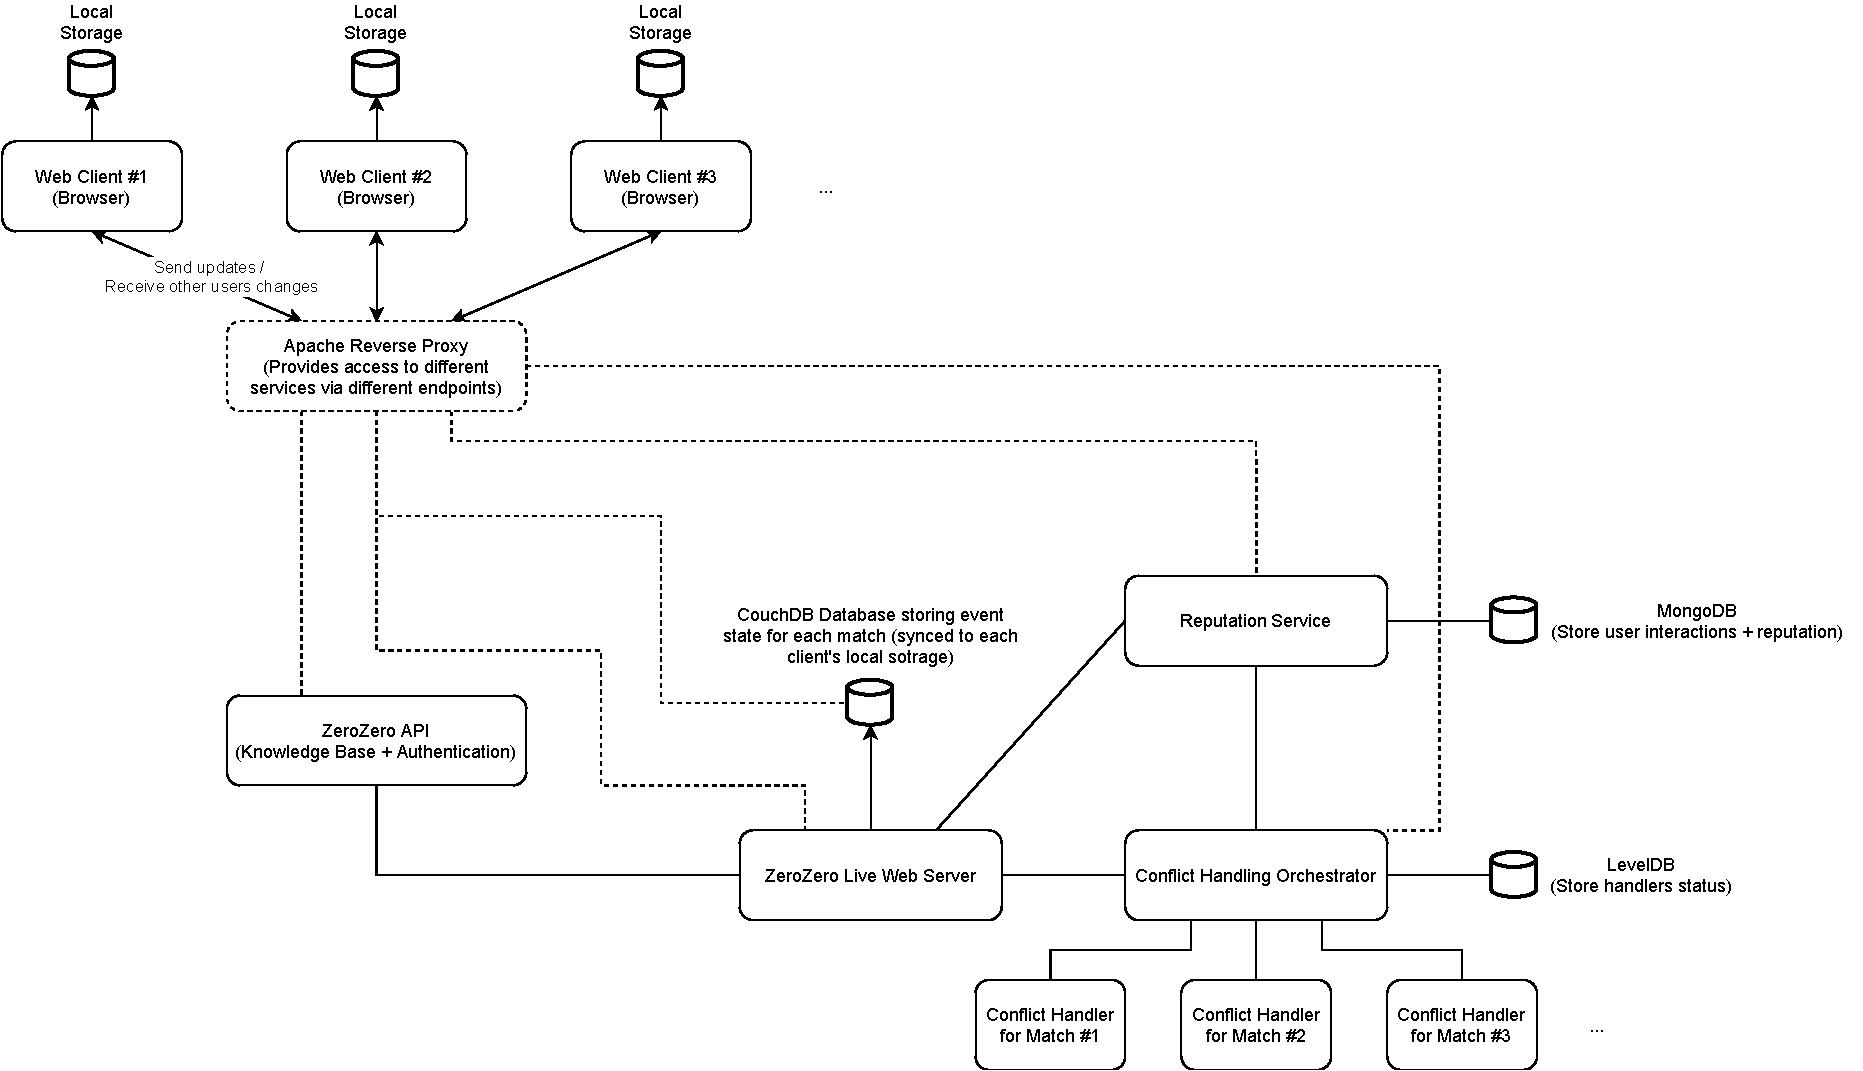
\includegraphics[height=0.9\textheight]{zerozerolive-arch.pdf}
        \caption{Services Architecture of the Application}
        \label{fig:annex-high-level-arch}
    \end{figure}
    \end{landscape}

\chapter{ZeroZero API events list} \label{annex:api-events}

\begin{longtable}{| p{.20\textwidth} | p{.60\textwidth} | p{.20\textwidth} |} 
    \caption{ZeroZero API events list (some fields were omitted for better reading purposes)} \\
    \hline
    \textbf{Event Id} & \textbf{Event Name} & \textbf{Category} \\ \hline
    \endfirsthead       
    \hline    
    \textbf{Event Id} & \textbf{Event Name} & \textbf{Category} \\ \hline       
    \endhead      
    8 & Estatísticas & 6 \\ \hline
    16 & Tempo Adicional & 6 \\ \hline
    24 & Info Jogador & 6 \\ \hline
    26 & Classificação & 6 \\ \hline
    29 & Outro Resultado & 6 \\ \hline
    43 & Lance polémico & 6 \\ \hline
    52 & VAR & 6 \\ \hline
    64 & Estatísticas Jogo & 6 \\ \hline
    78 & Fora de jogo & 6 \\ \hline
    79 & Castigado & 6 \\ \hline
    80 & Árbitros & 6 \\ \hline
    81 & Apresentação VAR & 6 \\ \hline
    83 & Canto & 6 \\ \hline
    3 & Comentário & 5 \\ \hline
    19 & Informação & 5 \\ \hline
    20 & Lesão grave & 5 \\ \hline
    22 & Homem do Jogo & 5 \\ \hline
    31 & Informação R. & 5 \\ \hline
    32 & Onzes Definidos & 5 \\ \hline
    36 & Info Pré-Jogo & 5 \\ \hline
    42 & Opinião & 5 \\ \hline
    46 & Antevisão & 5 \\ \hline
    47 & Rescaldo & 5 \\ \hline
    49 & Atualização de Resultado & 5 \\ \hline
    50 & Suplentes & 5 \\ \hline
    54 & Espetadores & 5 \\ \hline
    55 & Lesão & 5 \\ \hline
    5 & Substituição & 4 \\ \hline
    9 & Apito Inicial & 3 \\ \hline
    10 & Fim 1ª Parte & 3 \\ \hline
    11 & Início 2ª Parte & 3 \\ \hline
    12 & Fim 2ª Parte & 3 \\ \hline
    13 & Apito Final & 3 \\ \hline
    14 & Início Prolong. & 3 \\ \hline
    15 & Fim Prolong. & 3 \\ \hline
    56 & Fim 1ª Parte Prolongamento & 3 \\ \hline
    57 & Início 2ª Parte Prolongamento & 3 \\ \hline
    2 & Cartão Amarelo & 2 \\ \hline
    4 & Cartão Vermelho & 2 \\ \hline
    1 & Golo & 1 \\ \hline
    6 & Oportunidade Grande & 1 \\ \hline
    7 & Auto-Golo & 1 \\ \hline
    17 & Penalti Marcado & 1 \\ \hline
    18 & Penalti Falhado & 1 \\ \hline
    23 & Penalti Assin. & 1 \\ \hline
    35 & Penálti falhado & 1 \\ \hline
    44 & Golo invalidado & 1 \\ \hline
    53 & Oportunidade Pequena & 1 \\ \hline
    67 & Bola à barra & 1 \\ \hline
    68 & Bola ao poste & 1 \\ \hline
    84 & Assistência & 1 \\ \hline
    25 & Estatisticas 11 & 0 \\ \hline
    27 & Estatísticas Nac & 0 \\ \hline
    28 & Vídeo & 0 \\ \hline
    30 & Fotos & 0 \\ \hline
    34 & Penálti marcado & 0 \\ \hline
    37 & Info Pós-Jogo & 0 \\ \hline
    38 & JOG - Golos na Seleção (Único) & 0 \\ \hline
    39 & EQ - Resultados & 0 \\ \hline
    41 & Sondagem & 0 \\ \hline
    45 & Curiosidade PM & 0 \\ \hline
    48 & Fim de Relato & 0 \\ \hline
    51 & Bola ao ferro & 0 \\ \hline
    58 & Opinião com Foto & 0 \\ \hline
    60 & 5.ª falta & 0 \\ \hline
    61 & Time-out & 0 \\ \hline
    62 & Livre 10m assinalado & 0 \\ \hline
    63 & Cincos definidos & 0 \\ \hline
    65 & 5x4+GR & 0 \\ \hline
    66 & Faltas (Futsal) & 0 \\ \hline
    69 & Livre 10m Falhado & 0 \\ \hline
    70 & Livre 10m marcado & 0 \\ \hline
    71 & Livre direto assinalado & 0 \\ \hline 
    72 & Livre direto marcado & 0 \\ \hline
    73 & Livre direto falhado & 0 \\ \hline
    74 & 10.ª falta & 0 \\ \hline
    75 & 15.ª falta & 0 \\ \hline
    76 & 20.ª falta & 0 \\ \hline
    77 & Cartão Azul & 0 \\ \hline
    % \label{tab:myfirstlongtable}
\end{longtable}

% \begin{figure}[h]
%     \centering
%     \rotatebox{90}{
%         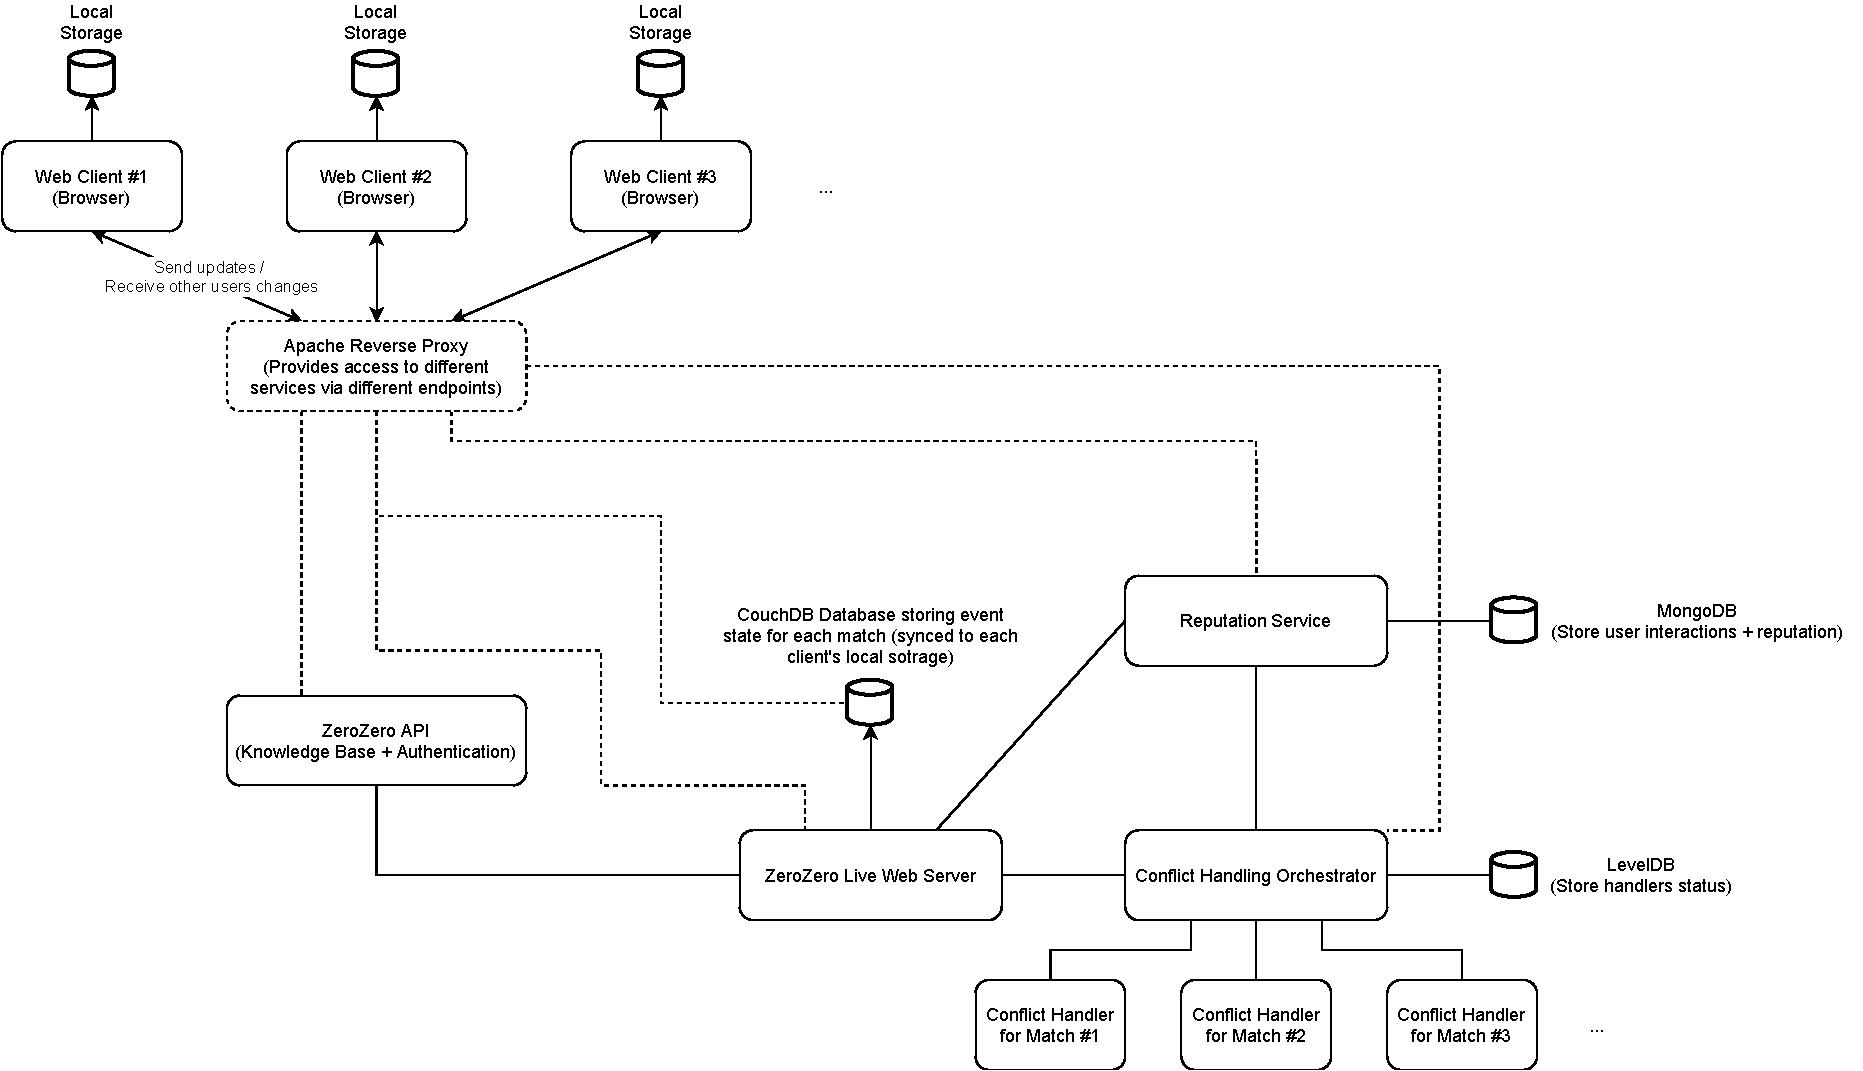
\includegraphics[width=0.5\textheight]{zerozerolive-arch.pdf}
%         % \caption{Services Architecture of the Application}
%     }

%     \end{figure}
    


\chapter{ZeroZero API events list} \label{annex:api-events}

\begin{longtable}{| p{.20\textwidth} | p{.60\textwidth} | p{.20\textwidth} |} 
    \caption{ZeroZero API events list (some fields were omitted for better reading purposes)} \\
    \hline
    \textbf{Event Id} & \textbf{Event Name} & \textbf{Category} \\ \hline
    \endfirsthead       
    \hline    
    \textbf{Event Id} & \textbf{Event Name} & \textbf{Category} \\ \hline       
    \endhead      
    8 & Estatísticas & 6 \\ \hline
    16 & Tempo Adicional & 6 \\ \hline
    24 & Info Jogador & 6 \\ \hline
    26 & Classificação & 6 \\ \hline
    29 & Outro Resultado & 6 \\ \hline
    43 & Lance polémico & 6 \\ \hline
    52 & VAR & 6 \\ \hline
    64 & Estatísticas Jogo & 6 \\ \hline
    78 & Fora de jogo & 6 \\ \hline
    79 & Castigado & 6 \\ \hline
    80 & Árbitros & 6 \\ \hline
    81 & Apresentação VAR & 6 \\ \hline
    83 & Canto & 6 \\ \hline
    3 & Comentário & 5 \\ \hline
    19 & Informação & 5 \\ \hline
    20 & Lesão grave & 5 \\ \hline
    22 & Homem do Jogo & 5 \\ \hline
    31 & Informação R. & 5 \\ \hline
    32 & Onzes Definidos & 5 \\ \hline
    36 & Info Pré-Jogo & 5 \\ \hline
    42 & Opinião & 5 \\ \hline
    46 & Antevisão & 5 \\ \hline
    47 & Rescaldo & 5 \\ \hline
    49 & Atualização de Resultado & 5 \\ \hline
    50 & Suplentes & 5 \\ \hline
    54 & Espetadores & 5 \\ \hline
    55 & Lesão & 5 \\ \hline
    5 & Substituição & 4 \\ \hline
    9 & Apito Inicial & 3 \\ \hline
    10 & Fim 1ª Parte & 3 \\ \hline
    11 & Início 2ª Parte & 3 \\ \hline
    12 & Fim 2ª Parte & 3 \\ \hline
    13 & Apito Final & 3 \\ \hline
    14 & Início Prolong. & 3 \\ \hline
    15 & Fim Prolong. & 3 \\ \hline
    56 & Fim 1ª Parte Prolongamento & 3 \\ \hline
    57 & Início 2ª Parte Prolongamento & 3 \\ \hline
    2 & Cartão Amarelo & 2 \\ \hline
    4 & Cartão Vermelho & 2 \\ \hline
    1 & Golo & 1 \\ \hline
    6 & Oportunidade Grande & 1 \\ \hline
    7 & Auto-Golo & 1 \\ \hline
    17 & Penalti Marcado & 1 \\ \hline
    18 & Penalti Falhado & 1 \\ \hline
    23 & Penalti Assin. & 1 \\ \hline
    35 & Penálti falhado & 1 \\ \hline
    44 & Golo invalidado & 1 \\ \hline
    53 & Oportunidade Pequena & 1 \\ \hline
    67 & Bola à barra & 1 \\ \hline
    68 & Bola ao poste & 1 \\ \hline
    84 & Assistência & 1 \\ \hline
    25 & Estatisticas 11 & 0 \\ \hline
    27 & Estatísticas Nac & 0 \\ \hline
    28 & Vídeo & 0 \\ \hline
    30 & Fotos & 0 \\ \hline
    34 & Penálti marcado & 0 \\ \hline
    37 & Info Pós-Jogo & 0 \\ \hline
    38 & JOG - Golos na Seleção (Único) & 0 \\ \hline
    39 & EQ - Resultados & 0 \\ \hline
    41 & Sondagem & 0 \\ \hline
    45 & Curiosidade PM & 0 \\ \hline
    48 & Fim de Relato & 0 \\ \hline
    51 & Bola ao ferro & 0 \\ \hline
    58 & Opinião com Foto & 0 \\ \hline
    60 & 5.ª falta & 0 \\ \hline
    61 & Time-out & 0 \\ \hline
    62 & Livre 10m assinalado & 0 \\ \hline
    63 & Cincos definidos & 0 \\ \hline
    65 & 5x4+GR & 0 \\ \hline
    66 & Faltas (Futsal) & 0 \\ \hline
    69 & Livre 10m Falhado & 0 \\ \hline
    70 & Livre 10m marcado & 0 \\ \hline
    71 & Livre direto assinalado & 0 \\ \hline 
    72 & Livre direto marcado & 0 \\ \hline
    73 & Livre direto falhado & 0 \\ \hline
    74 & 10.ª falta & 0 \\ \hline
    75 & 15.ª falta & 0 \\ \hline
    76 & 20.ª falta & 0 \\ \hline
    77 & Cartão Azul & 0 \\ \hline
    % \label{tab:myfirstlongtable}
\end{longtable}
\chapter{ZeroZero Live Frontend Interfaces}

\begin{figure}[h]
    \begin{center}
        \leavevmode
        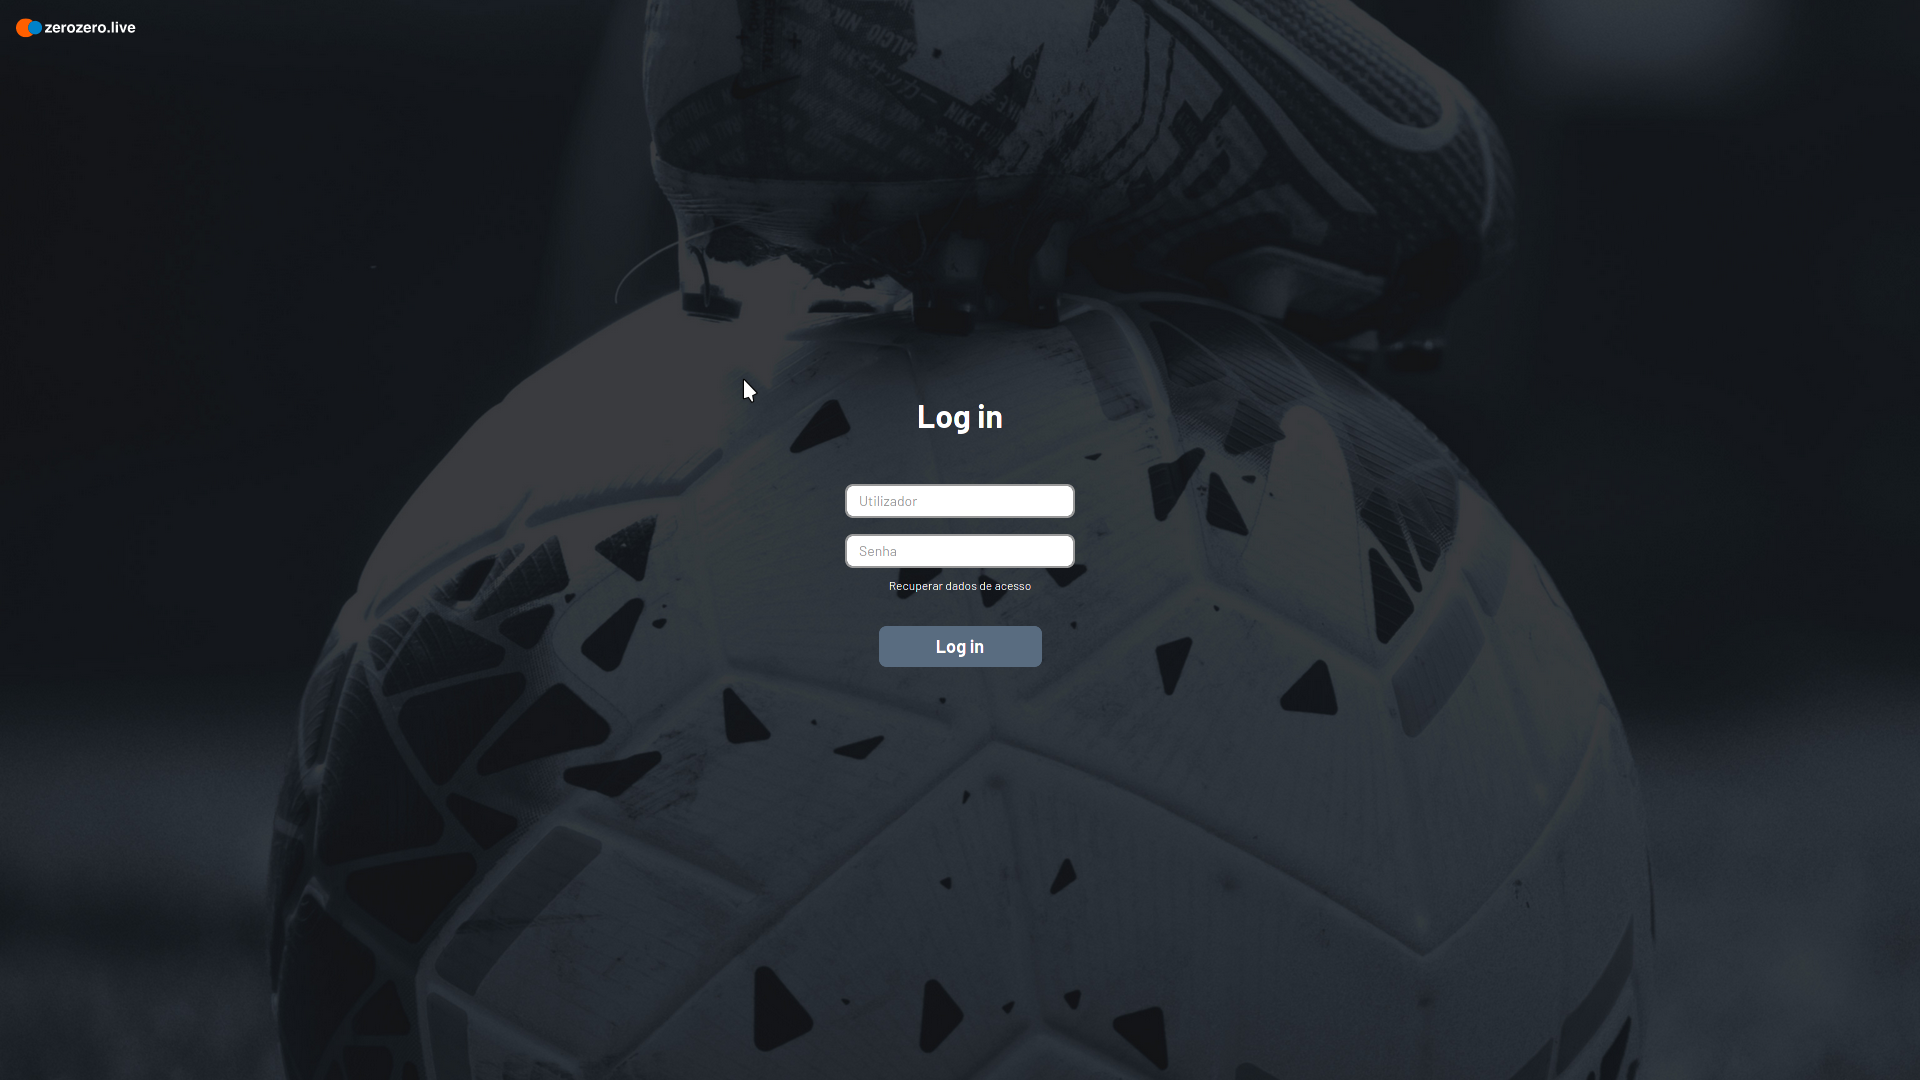
\includegraphics[width=\textwidth]{zerozerolive-login.png}
        \caption{Login page of zerozero.live}
        \label{fig:zerozerolive-login}
    \end{center}
\end{figure}

\begin{figure}
    \begin{center}
        \leavevmode
        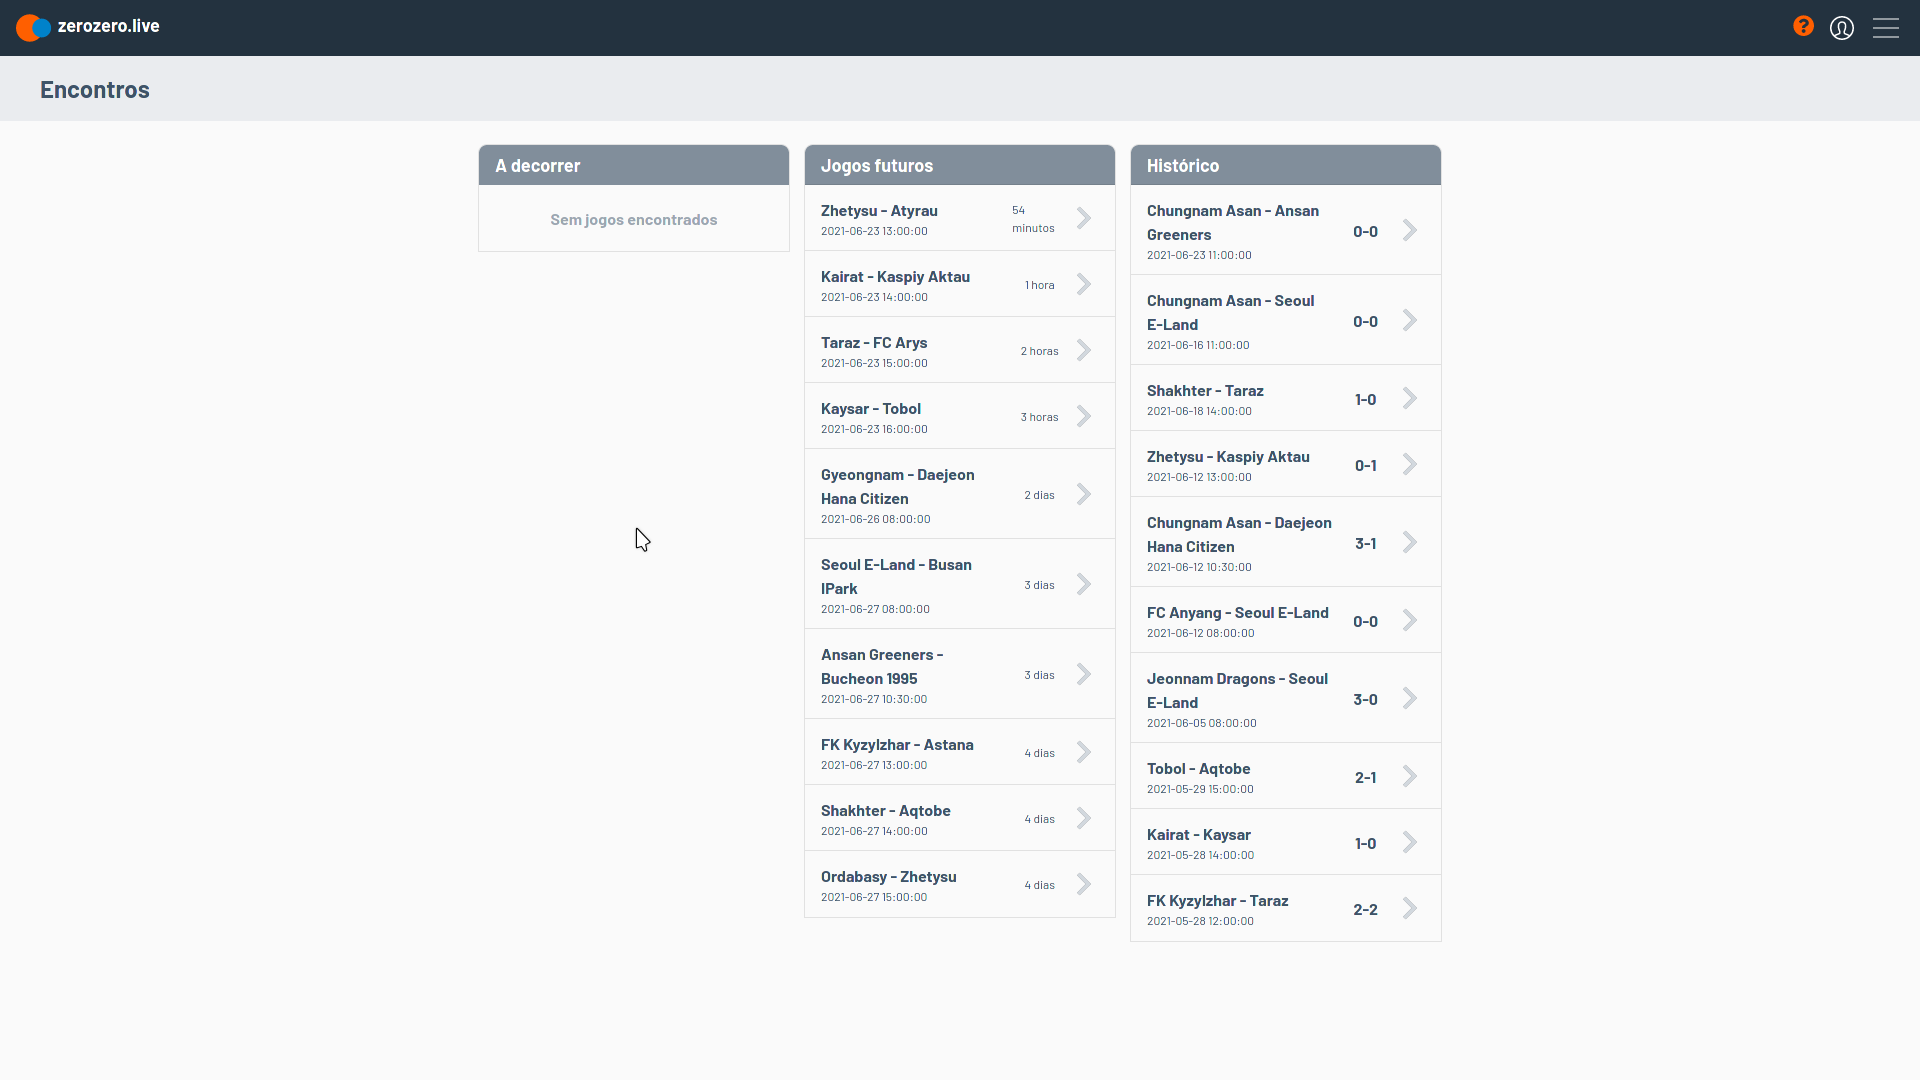
\includegraphics[width=\textwidth]{zerozerolive-home.png}
        \caption{Homepage of zerozero.live}
        \label{fig:zerozerolive-home}
    \end{center}
\end{figure}

\begin{figure}
    \begin{center}
        \leavevmode
        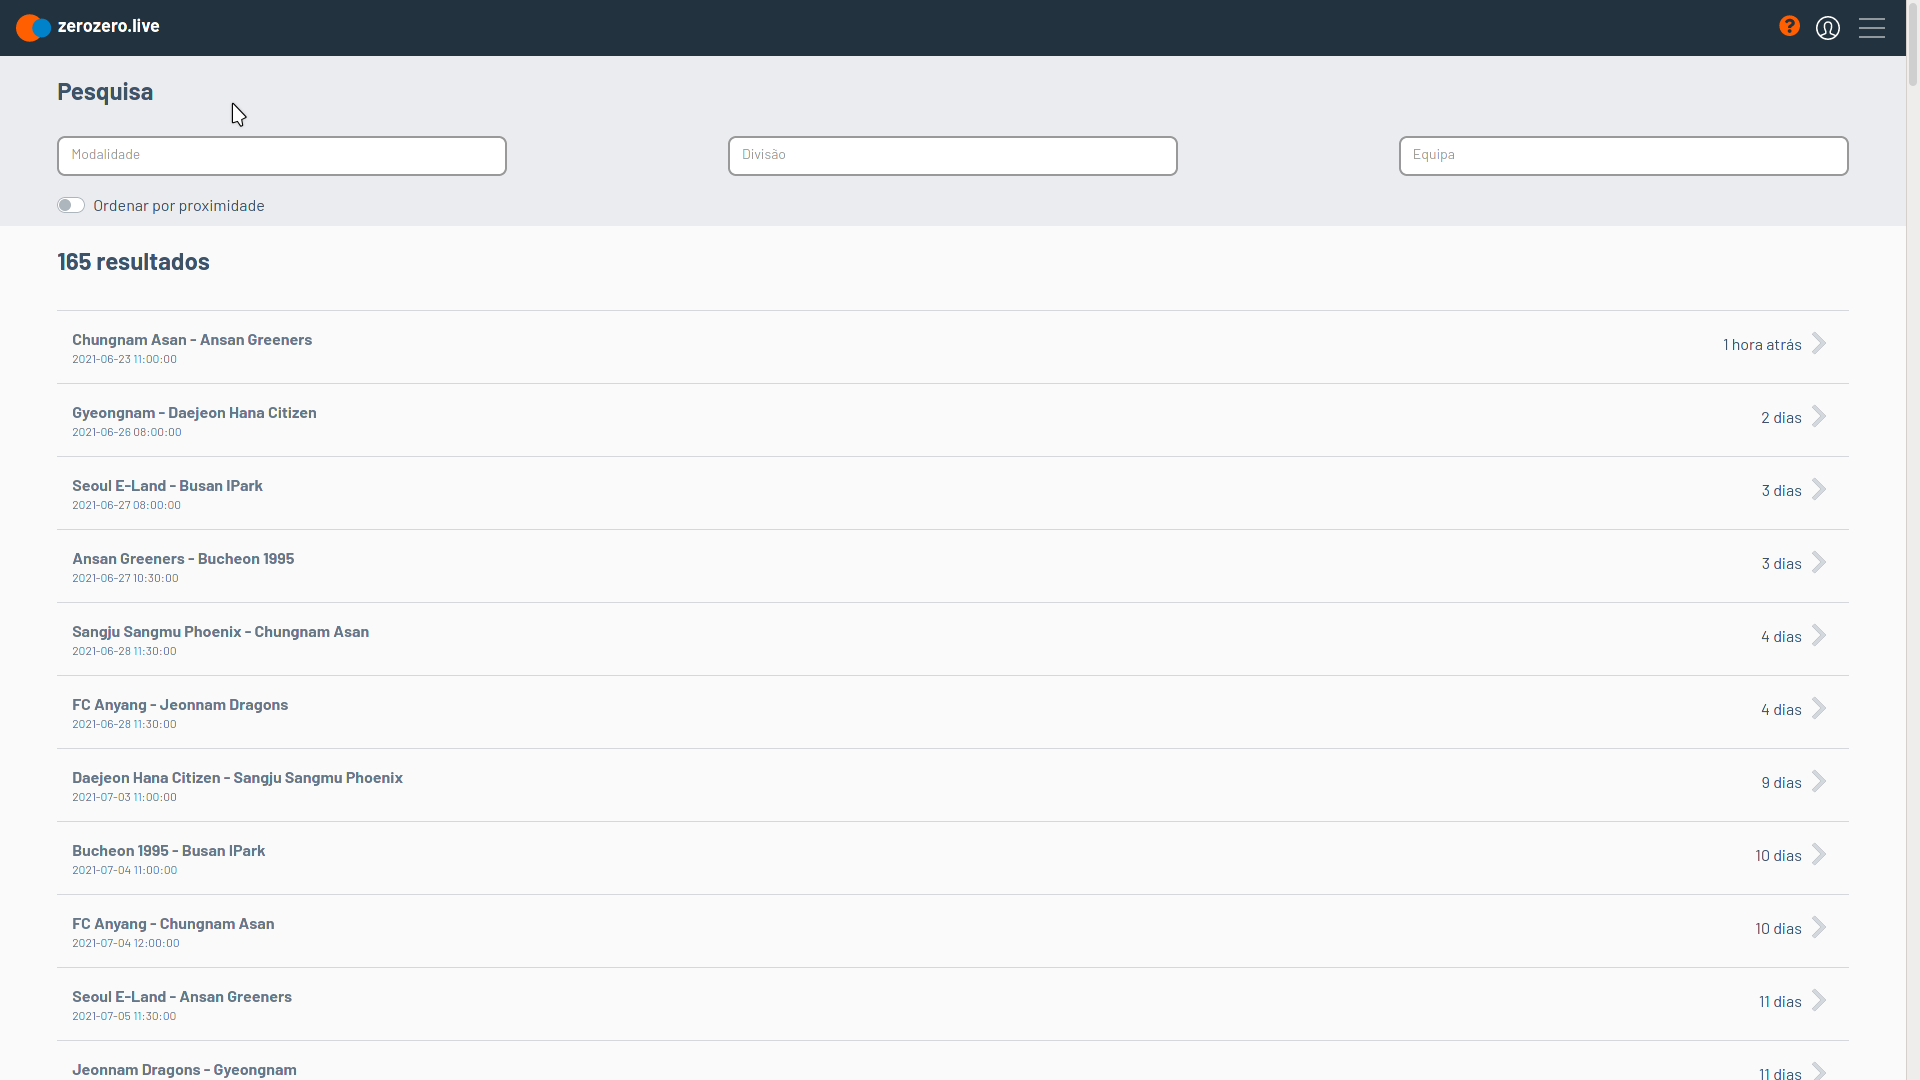
\includegraphics[width=\textwidth]{zerozerolive-search.png}
        \caption{Search page of zerozero.live}
        \label{fig:zerozerolive-search}
    \end{center}
\end{figure}

\begin{figure}
    \begin{center}
        \leavevmode
        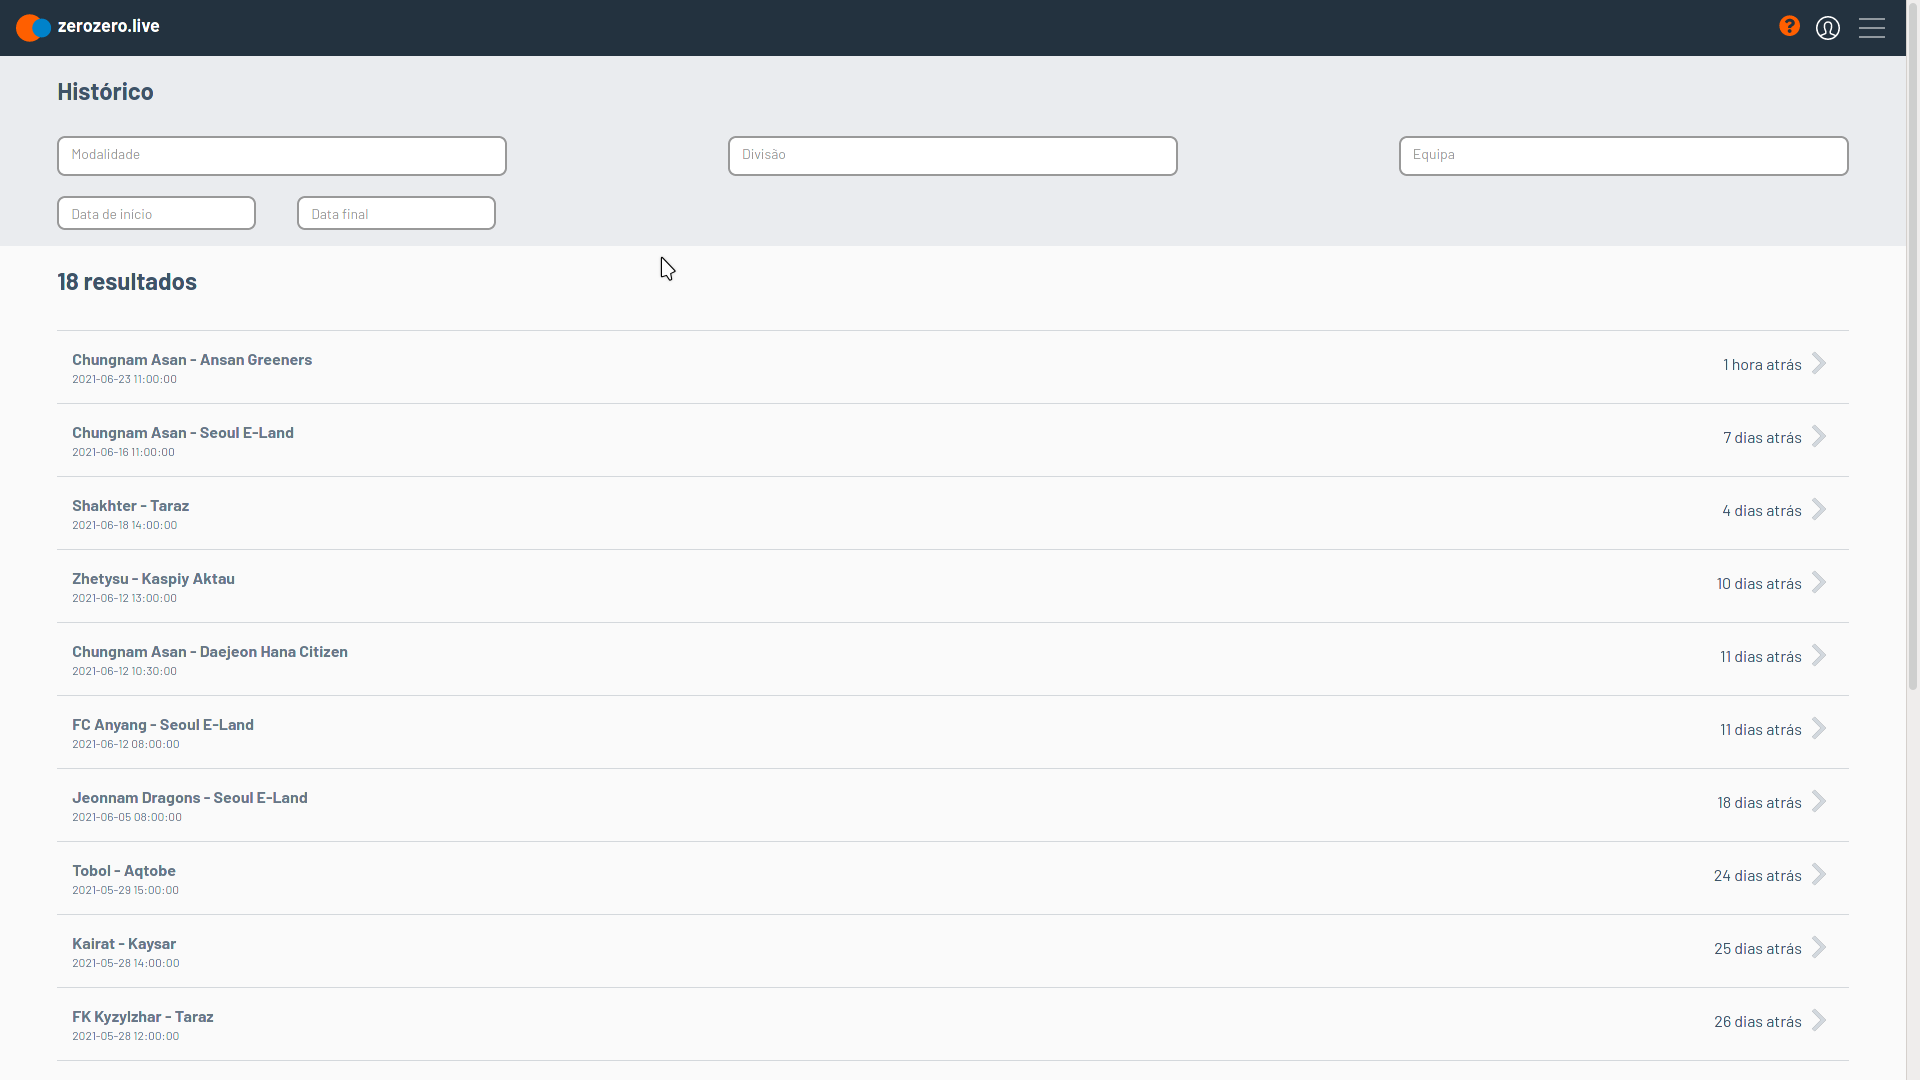
\includegraphics[width=\textwidth]{zerozerolive-history.png}
        \caption{History page of zerozero.live}
        \label{fig:zerozerolive-history}
    \end{center}
\end{figure}

\begin{figure}
    \begin{center}
        \leavevmode
        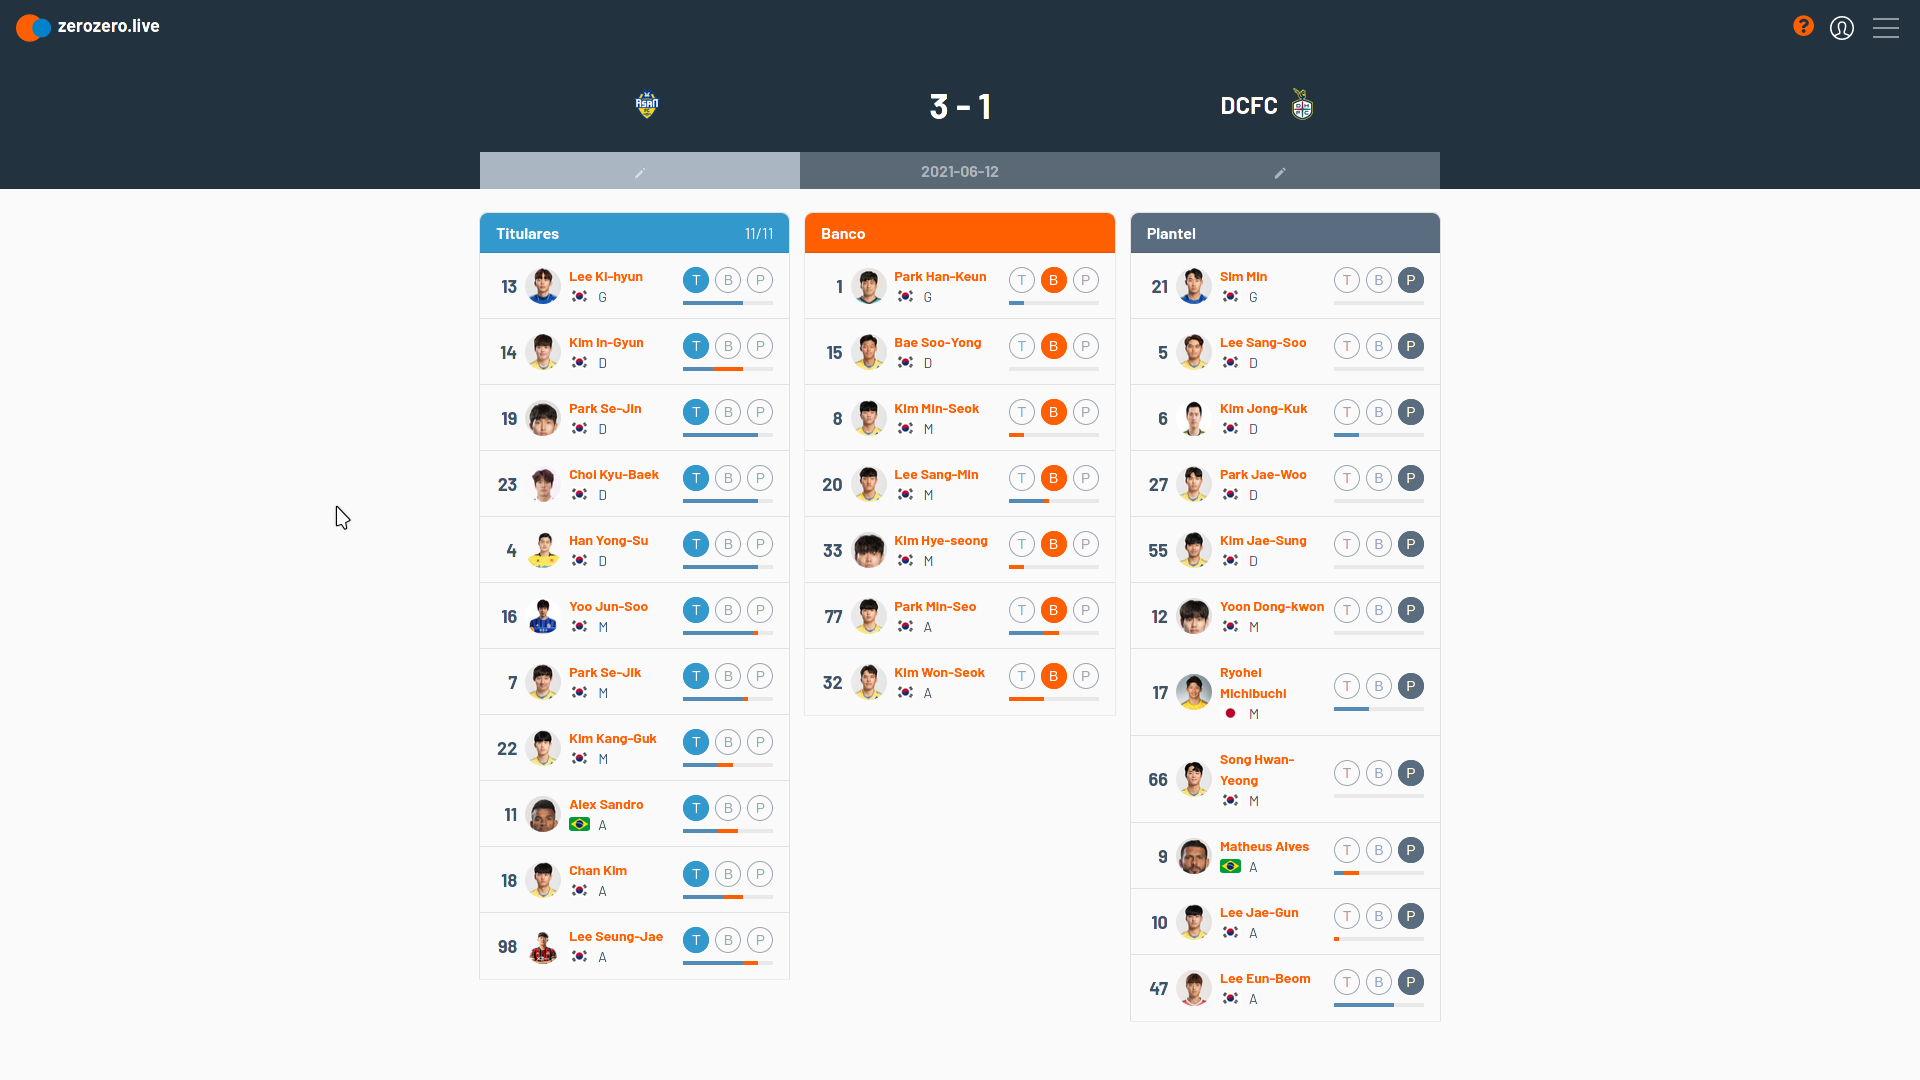
\includegraphics[width=\textwidth]{zerozerolive-teams.png}
        \caption{Team selection for a match in zerozero.live}
        \label{fig:zerozerolive-teams}
    \end{center}
\end{figure}

\begin{figure}[h]
    \begin{center}
        \leavevmode
        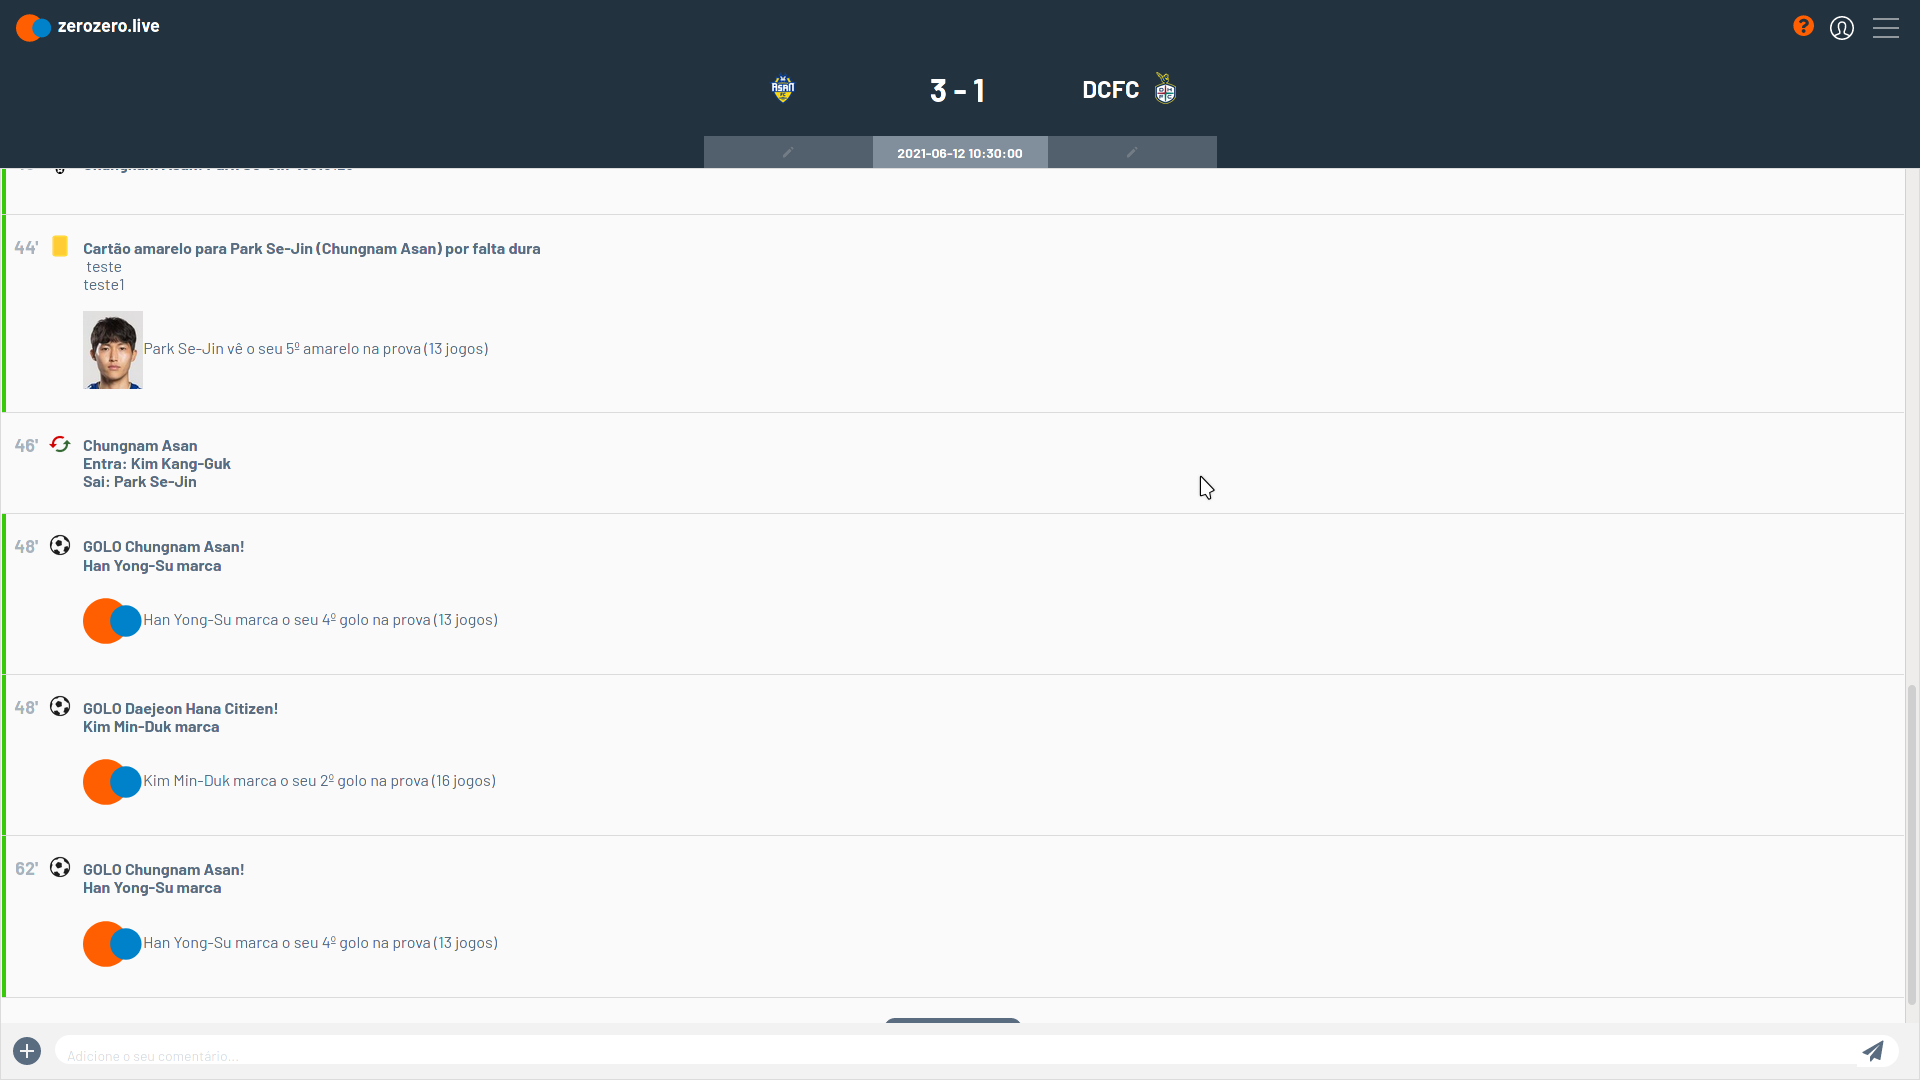
\includegraphics[width=\textwidth]{zerozerolive-comments.png}
        \caption{Comments page for a match in zerozero.live}
        \label{fig:annex-zerozerolive-comments}
    \end{center}
\end{figure}

%% Index
%% Uncomment next command if index is required
%% don't forget to run ``makeindex thesis'' command
%\PrintIndex

\end{document}
